

\documentclass[a4paper,8pt]{extarticle} % extarticle allows to use font size of 8pt.

\usepackage[a4paper, top=1.6cm, bottom=2cm, left=1.6cm, right=1.6cm]{geometry} % Marge reduction.

%% Language specific package
\usepackage[french]{babel}
\frenchbsetup{StandardLists=true} % Necessary to use enumitem with babel/french.

%% Font and typing packages
\usepackage{fontspec}
\setmainfont[
	Ligatures=TeX,
	ItalicFont={Dancing Script},
	BoldItalicFont={Dancing Script}
	]{PT Serif} % default is Latin Modern
\newfontfamily\antiquefont[Ligatures=TeX]{Caslon Antique} % fancy font
\usepackage{microtype}			% Greatly improves general appearance of the text.
\usepackage{SIunits}			% Unit appearance.
\usepackage{xspace}				% Define commands that appear not to eat spaces.
\usepackage{ulem}				% To cross words out. Use \sout{}.

%% Array utilities
\usepackage{array}				% Additionnal options for arrays.
\usepackage{colortbl}			% Additionnal options for coloring arrays.
\usepackage[table]{xcolor}		% Auto alternate grey-white rows.
\usepackage[export]{adjustbox}		% Centered pics in tables

%% List utilities
\usepackage[inline]{enumitem}   % Display inline lists.
\usepackage{etoolbox}           % General utility. Good for lists for instance.
\usepackage{xparse}             % List utilities.
\usepackage{datatool}	% Handling alphabetical order.

%% Frames
\usepackage{framed}				% Boxes.
\usepackage[framemethod=TikZ]{mdframed}% For fancy frames.
\usepackage{tikz}				% For fancy frames.
\usepackage{wrapfig}			% Fancy insertion of pics in text.

%% Page utilities
\usepackage{multicol}			% Allows to divide a part of the page in multiple columns.
	
%% Others
\usepackage{keyval}             % Used to create maps of commands/labels/objects.
	\makeatletter                  % Mandatory for the usage of keyval.
\usepackage{xstring}            % String parsing, cutting, etc.
\usepackage{hyperref} % Links in PDF.


%%% Update of the dotfill command to always get dots

\newcommand{\predotfill}{\penalty0\hbox{}\nobreak}%


%%% Command to avoid typing \xspace when creating a new name macro

\newcommand{\newnamemacro}[2]{\newcommand{#1}{#2}} % \xspace removed for compatibility with alphabetical ordering

%%% Language specific stuff


\newcommand{\translationteam}{\item \og AEnoriel \fg \item \og Anglachel \fg \item \og Astadriel \fg \item \og Batcat \fg \item \og Bigfish \fg \item \og Eru \fg  \item \og Gandarin \fg \item \og Groumbahk \fg \item \og Iluvatar \fg \item \og Mammstein \fg \item \og Shlagrabak \fg \item et beaucoup d'autres...}

\hypersetup{
	pdfauthor={Équipe de traduction française de T9A},
	pdfsubject={Règles pour le jeu Batailles Fantastiques : Le 9\ieme{} Âge},
}

%%% Commands %%%

\ifdef{\isitanAB}{

\newcommand{\addtosortedlist}[1]{%
	\protected@edef\textarg{#1}%
	\protected@edef\textwithoutspaces{\expandafter\removespaces\expandafter{\textarg}}%
	\substitute\textwithoutspaces{É}{E}% Most used special characters of the language, and equivalent for alphabetical ordering
	\substitute\textwithoutspaces{È}{E}%
	\substitute\textwithoutspaces{Ê}{E}%
	\substitute\textwithoutspaces{é}{e}%
	\substitute\textwithoutspaces{è}{e}%
	\substitute\textwithoutspaces{ê}{e}%
	\substitute\textwithoutspaces{À}{A}%
	\substitute\textwithoutspaces{à}{a}%
	\substitute\textwithoutspaces{ù}{u}%
	\expandafter\sortitem\expandafter[\textwithoutspaces]{#1}%
}%

\newcommand{\pts}[1]{% First step is to remove spaces if there are some
	\def\numberwithoutspaces{\expandafter\removespaces\expandafter{#1}}%
	% Next step is getting rid of formatting if there are any (bold, color, ...)
	\pdfstringdef\cleannumber{\numberwithoutspaces}%
	% Now we can try if it is 1 or not
	\expandafter\ifstrequal\expandafter{\cleannumber}{1}{#1~\labels@point}{%
	\expandafter\ifstrequal\expandafter{\cleannumber}{0.5}{0,5~\labels@point}{%
	\expandafter\ifstrequal\expandafter{\cleannumber}{1.5}{1,5~\labels@point}{%
	#1~\labels@points}}}%
}

}{}

% Dark gods
\newcommand{\dchange}{Changement}
\newcommand{\dlust}{Luxure}
\newcommand{\pestilence}{Pestilence}
\newcommand{\wrath}{Courroux}
\newcommand{\truechaos}{Chaos Primordial}


% Nothing to edit here

\ifdef{\isitanAB}{

\newcommand{\alliancepts}[1]{
\ifsubstring{#1}{\free}{%
		\free{}%
	}{%
	\ifsubstring{#1}{\permodel}{%
		\splitatinf{#1}\myoption\myvalue%
		\pts{\myvalue}\permodel{}%
	}{%
	\pts{#1}
	}}
}

% You might wanna change the order of the gods - advanced user
\newcommand{\allianceoptions}[1]{%
	\defallianceoptions{#1}%
	\unitentryformat{\labels@allianceoptions\spacebeforecolon{}:}\newline
	\expandafter\ifblank\expandafter{\allianceoptions@introsentence}{}{\noindent\allianceoptions@introsentence{}\spacebeforecolon{}:}
	
	\expandafter\ifblank\expandafter{\allianceoptions@wrath}{
		\setlength{\columnseprule}{0.5pt}
		\renewcommand{\columnseprulecolor}{\color{black!30}}
		\vspace*{-0.2cm}\begin{multicols}{3}\raggedcolumns
		
			\begin{center}
			\noindent\dchange{}
			
			\noindent\alliancepts{\allianceoptions@change}
			\vspace*{-0.3cm}
			\end{center}
		
		\columnbreak
		
			\begin{center}
			\noindent\dlust{}
			
			\noindent\alliancepts{\allianceoptions@lust}
			\vspace*{-0.3cm}
			\end{center}
		
		\columnbreak

			\begin{center}
			\noindent\pestilence{}
			
			\noindent\alliancepts{\allianceoptions@pestilence}
			\vspace*{-0.3cm}
			\end{center}
			
		\end{multicols}
		\setlength{\columnseprule}{0pt}	
	}{
		\setlength{\columnseprule}{0.5pt}
		\renewcommand{\columnseprulecolor}{\color{black!30}}
		\vspace*{-0.2cm}\begin{multicols}{4}\raggedcolumns
		
			\begin{center}
			\noindent\dchange{}
			
			\noindent\alliancepts{\allianceoptions@change}
			\vspace*{-0.3cm}
			\end{center}
		
		\columnbreak

			\begin{center}
			\noindent\wrath{}
			
			\noindent\alliancepts{\allianceoptions@wrath}
			\vspace*{-0.3cm}
			\end{center}
		
		\columnbreak
		
			\begin{center}
			\noindent\dlust{}
			
			\noindent\alliancepts{\allianceoptions@lust}
			\vspace*{-0.3cm}
			\end{center}
		
		\columnbreak

			\begin{center}
			\noindent\pestilence{}
			
			\noindent\alliancepts{\allianceoptions@pestilence}
			\vspace*{-0.3cm}
			\end{center}
			
		\end{multicols}
		\setlength{\columnseprule}{0pt}
	}
}

}{}


%%% Labels %%%

% Profile

\newcommand{\labels@M}{M}
\newcommand{\labels@WS}{CC}
\newcommand{\labels@BS}{CT}
\newcommand{\labels@S}{F}
\newcommand{\labels@T}{E}
\newcommand{\labels@W}{PV}
\newcommand{\labels@I}{I}
\newcommand{\labels@A}{A}
\newcommand{\labels@Ld}{Cd}
\newcommand{\labels@Invocation}{Invocation} % For Vampire Covenant profiles
\newcommand{\labels@roundbase}{rond} % printed after XX mm for round bases

\newcommand{\Strength}{Force}

% Technical

\newcommand{\labels@range}{Portée}
\newcommand{\labels@point}{pt}
\newcommand{\labels@points}{pts}
\newcommand{\labels@only}{uniquement}
\newcommand{\labels@magic}{Magie}
\newcommand{\labels@pathsused}{Génère ses sorts dans la Discipline}
\newcommand{\labels@model}{figurine}
\newcommand{\labels@models}{figurines}
\newcommand{\labels@Singlemodel}{Figurine \textbf{seule}}

% Unit entry labels

\newcommand{\labels@basesize}{Socle}
\newcommand{\labels@trooptype}{Type de troupe}
\newcommand{\labels@specialrules}{Règles Spéciales}
\newcommand{\labels@alignment}{Allégeance}
\newcommand{\labels@alliance}{Allégeance}
\newcommand{\labels@allianceoptions}{Options d'Allégeance}
\newcommand{\labels@greenhiderace}{Race de Peaux Vertes}
\newcommand{\labels@equipment}{Équipement}
\newcommand{\labels@weapons}{Armes}
\newcommand{\labels@armour}{Armure}
\newcommand{\labels@options}{Options}
\newcommand{\labels@commandgroup}{État-Major}
\newcommand{\labels@charactermounts}{Montures de Personnages}
\newcommand{\labels@mounts}{Montures}
\newcommand{\labels@mount}{Monture}
\newcommand{\labels@specialequipment}{Équipement Spécial}

% Command groups

\newcommand{\labels@champion}{Champion}
\newcommand{\labels@standardbearer}{Porte-Étendard}
\newcommand{\labels@musician}{Musicien}
\newcommand{\labels@singlebannerallowance}{Une seule unité de ce type peut prendre une Bannière Magique}
\newcommand{\labels@condsinglebannerallowance}{Une seule unité de ce type peut prendre une Bannière Magique si}
\newcommand{\labels@bannerallowance}{Bannière Magique}
\newcommand{\labels@veteranstandardbearer}{Peut devenir Porte-Étendard Vétéran}
\newcommand{\labels@championallowance}{Arme Magique}

% Titles

\newcommand{\labels@armylist}{Liste des Troupes}
\newcommand{\labels@lords}{Seigneurs}
\newcommand{\labels@heroes}{Héros}
\newcommand{\labels@coreunits}{Unités de Base}
\newcommand{\labels@specialunits}{Unités Spéciales}
\newcommand{\labels@rareunits}{Unités Rares}
\newcommand{\labels@armywiderules}{Règles Communes de l'Armée}
\newcommand{\labels@armyspecialrules}{Règles Spéciales de l'Armée}
\newcommand{\labels@armoury}{Armurerie}
\newcommand{\labels@magicalitems}{Objets Magiques}
\newcommand{\labels@magicalweapons}{Armes Magiques}
\newcommand{\labels@magicalarmour}{Armures Magiques}
\newcommand{\labels@talismans}{Talismans}
\newcommand{\labels@enchanteditems}{Objets Enchantés}
\newcommand{\labels@arcaneitems}{Objets Cabalistiques}
\newcommand{\labels@magicalbanners}{Bannières Magiques}
\newcommand{\labels@quickrefsheet}{Fiche de Référence}
\newcommand{\labels@changelog}{Change Log}

\newcommand{\labels@lordsInitial}{S}
\newcommand{\labels@heroesInitial}{H}
\newcommand{\labels@coreunitsInitial}{B}
\newcommand{\labels@specialunitsInitial}{S}
\newcommand{\labels@rareunitsInitial}{R}
\newcommand{\labels@mountsInitial}{M}


% Titlepage

\newcommand{\labels@fantasybattles}{Batailles Fantastiques}
\newcommand{\labels@NinthAge}{Le 9\ieme{} Âge}
\newcommand{\labels@armyrules}{Règles de l'Armée}
\newcommand{\labels@frontpagecredits}{%
\labels@fantasybattles{} : \labels@NinthAge{} est un jeu créé et entretenu par la communauté qui met en scène des affrontements de figurines.\newline
Toutes les règles sont disponibles gratuitement sur le site suivant. Vos retours et suggestions sont les bienvenus : \url{http://www.the-ninth-age.com/}
}
\newcommand{\labels@license}{Copyright Creative Commons license : \url{the-ninth-age.com/license.html}}
\newcommand{\labels@tableofcontents}{Sommaire}
\newcommand{\labels@introduction}{%
\begin{center}\noindent{\Largerfontsize\textbf{Note des traducteurs}}\end{center}
\vspace{0.5cm}

Nous souhaitons remercier chaleureusement l'équipe à l'initiative du 9\ieme{} Âge pour leur motivation et leur travail continu pour faire vivre notre passion. Nous espérons que ce jeu saura développer les qualités pour plaire au plus grand nombre et réunir les joueurs, amateurs comme habitués des tournois, autour de règles amusantes et équilibrées, pour finalement s'imposer comme un standard du jeu de figurines. Une grande ambition qui ne pourra s'accomplir que \textbf{grâce à vous}, la communauté, via des retours constructifs, afin de modeler le jeu selon nos désirs. N'étant \textbf{en aucun cas à but lucratif}, le 9\ieme{} Âge part avec un avantage considérable. Les règles des éventuelles nouvelles sorties ne sont pas dictées par le besoin de vendre ces nouveautés. Vous pouvez choisir et acheter vos figurines où bon vous semble, il n'y a pas un unique revendeur toléré. Enfin, vous pouvez être assurés que tant que le 9\ieme{} Âge sera joué, vous disposerez d'un \textbf{support continu et régulier}, celui-ci étant offert par la communauté.

Concernant la traduction en elle-même, nous avons fait de notre mieux pour vous offrir une version de qualité, dont nous espérons qu'elle surpasse celle de la version originale ! Si vous constatez des coquilles, des erreurs, merci de nous les signaler en nous contactant sur le forum du 9\ieme{} Âge, dans le \textbf{sous-forum français} (\url{http://www.the-ninth-age.com/index.php?board/117-french/}). Vous y trouverez aussi les dernières mises à jour. \textbf{En cas de conflit d'interprétation avec la version originale, la version originale fait référence}.

\vspace{0.5cm}
Que ce jeu vous apporte d'innombrables heures de plaisir partagé !

\vspace{1cm}

\ifdef{\translationteam}{
	\begin{multicols}{3}
	\begin{itemize}
		\translationteam
	\end{itemize}
	\end{multicols}
}{}
}
\newcommand{\labels@rulechanges}{% blank ATM
}
\newcommand{\labels@latexcredit}{Document réalisé à l'aide de \LaTeX .}


%%% Technical commands

\newcommand{\only}[1]{(#1 uniquement)}
\newcommand{\free}{gratuit}
\newcommand{\upto}{jusqu'à}
\newcommand{\Upto}{Jusqu'à}
\newcommand{\unlimited}{pas de limite}
\newcommand{\permodel}{/fig.}
\newcommand{\listlastchoice}{ ou}
\newcommand{\notif}[1]{(pas #1)}
\newcommand{\wordand}{et}
\newcommand{\wordwith}{avec}
\newcommand{\ifNmodelsorless}[1]{(#1 figurines ou moins)}
\newcommand{\unitwith}{unité avec}
\newcommand{\From}{De} % From ... to ... models
\newcommand{\wordto}{à}
\newcommand{\wordAll}{Tous}
\newcommand{\spacebeforecolon}{ } % French put a space before colons
\newcommand{\minprice}{Coût min. :}
\newcommand{\mincostfor}{Coût min. pour}
\newcommand{\maxunitsize}{Taille max.}
\newcommand{\additionalfigscost}{Les figurines additionnelles coûtent}


%%% Special rules %%%

\newcommand{\ambush}{Embuscade}
\newcommand{\armourpiercing}[1]{Perforant\ifblank{#1}{}{ (#1)}}
\newcommand{\bodyguard}[1]{Garde du Corps\ifblank{#1}{}{ (#1)}}
\newcommand{\breathweapon}[1]{Attaque de Souffle\ifblank{#1}{}{ (#1)}}
\newcommand{\channel}{Canalisation}
\newcommand{\crushattack}{Attaque Écrasante}
\newcommand{\daemonicinstability}{Instabilité Démoniaque}
\newcommand{\devastatingcharge}{Charge Dévastatrice}
\newcommand{\distracting}{Distrayant}
\newcommand{\divineattacks}{Attaques Divines}
\newcommand{\engineer}{Ingénieur}
\newcommand{\ethereal}{Éthéré}
\newcommand{\fastcavalry}{Cavalerie Légère}
\newcommand{\fear}{Peur}
\newcommand{\fightinextrarank}{Combat avec un Rang Supplémentaire}
\newcommand{\fireborn}{Né du Feu}
\newcommand{\flamingattacks}{Attaques Enflammées}
\newcommand{\flammable}{Inflammable}
\newcommand{\frenzy}{Frénésie}
\newcommand{\fly}[1]{Vol\ifblank{#1}{}{ (#1)}}
\newcommand{\grindingattacks}[1]{Attaques de Broyage\ifblank{#1}{}{ (#1)}}
\newcommand{\hardtarget}{Camouflé}
\newcommand{\hatred}{Haine}
\newcommand{\hellfire}{Feu Démoniaque}
\newcommand{\hidden}{Caché}
\newcommand{\holyattacks}{Attaques Divines} % deprecated, still has to be filled. same as Divine Attacks.
\newcommand{\immunetopsychology}{Immunisé à la Psychologie}
\newcommand{\impacthits}[1]{Touches d'Impact\ifblank{#1}{}{ (#1)}}
\newcommand{\insignificant}{Insignifiant}
\newcommand{\largetarget}{Grande Cible}
\newcommand{\lethalstrike}{Coup Fatal}
\newcommand{\lightningattacks}{Attaques Foudroyantes}
\newcommand{\lightningreflexes}{Réflexes Foudroyants}
\newcommand{\lighttroops}{Troupe Légère}
\newcommand{\magicresistance}[1]{Résistance à la Magie\ifblank{#1}{}{ (#1)}}
\newcommand{\magicalattacks}{Attaques Magiques}
\newcommand{\metalshifting}{Fusion du Métal}
\newcommand{\moveorfire}{Mouvement ou Tir}
\newcommand{\multipleshots}[1]{Tirs Multiples\ifblank{#1}{}{ (#1)}}
\newcommand{\multiplewounds}[2]{Blessures Multiples\ifblank{#1}{}{ (#1\ifblank{#2}{)}{, #2)}}}
\newcommand{\notaleader}{Pas un Meneur}
\newcommand{\otherworldly}{D'Outre-Monde}
\newcommand{\pathmaster}[1]{Maître de la Voie\ifblank{#1}{}{ (#1)}}
\newcommand{\poisonedattacks}{Attaques Empoisonnées}
\newcommand{\quicktofire}{Tir Rapide}
\newcommand{\randommovement}[1]{Mouvement Aléatoire\ifblank{#1}{}{ (#1)}}
\newcommand{\randomattacks}[1]{Attaques Aléatoires\ifblank{#1}{}{ (#1)}}
\newcommand{\regeneration}[1]{Régénération\ifblank{#1}{}{ (#1+)}}
\newcommand{\reload}{Rechargez !}
\newcommand{\requirestwohands}{Arme à deux Mains}
\newcommand{\scythes}{Faux}
\newcommand{\scout}{Éclaireur}
\newcommand{\scouts}{Éclaireurs}
\newcommand{\stomp}[1]{Piétinement\ifblank{#1}{}{ (#1)}}
\newcommand{\strider}[1]{Guide\ifblank{#1}{}{ (#1)}}
\newcommand{\stubborn}{Tenace}
\newcommand{\stupidity}{Stupidité}
\newcommand{\skirmisher}{Tirailleur}
\newcommand{\skirmishers}{Tirailleurs}
\newcommand{\sweepingattack}{Attaque au Passage}
\newcommand{\swiftstride}{Course Rapide}
\newcommand{\thunderouscharge}{Charge Tonitruante}
\newcommand{\terror}{Terreur}
\newcommand{\toxicattacks}{Attaques Toxiques}
\newcommand{\unbreakable}{Indémoralisable}
\newcommand{\undead}{Mort-Vivant}
\newcommand{\unstable}{Instable}
\newcommand{\unwieldy}{Encombrant}
\newcommand{\vanguard}{Avant-Garde}
\newcommand{\volleyfire}{Tir de Volée}
\newcommand{\warplatform}{Plateforme de Guerre}
\newcommand{\wardsave}[1]{Sauvegarde Invulnérable\ifblank{#1}{}{ (#1+)}}
\newcommand{\weaponmaster}{Maître d'Ar\-mes}
\newcommand{\wizardconclave}[1]{Conclave de Sorciers\ifblank{#1}{}{ (#1)}}


%%% Magic %%%


% General

\newcommand{\Pathof}{Voie}

\newcommand{\battle}{Commune}

\newcommand{\anyofthebattlemagic}{dans n'importe laquelle des Voies Communes}
\newcommand{\ONLYanyofthebattlemagic}{Commune de votre choix}

\newcommand{\magiclevel}[1]{\ifnumcomp{#1}{<}{3}{Apprenti Magicien}{Maître Magicien} Niveau #1}
\newcommand{\Level}{Niveau}

\newcommand{\wizard}{Magicien}
\newcommand{\wizards}{Magiciens}

\newcommand{\learnedspell}{Sort Appris}
\newcommand{\learnedspells}{Sorts Appris}
\newcommand{\attributespell}{Attribut de la Voie}
\newcommand{\attributespells}{Attributs de la Voie}
\newcommand{\attributespellnumber}{A}
\newcommand{\traitspell}{Sort Caractéristique}
\newcommand{\traitspells}{Sorts Caractéristiques}
\newcommand{\traitspellnumber}{C}


\newcommand{\boundspell}[1]{Objet de Sort\ifblank{#1}{}{, Puissance #1}}
\newcommand{\boundspells}[1]{Objets de Sort\ifblank{#1}{}{, Puissance #1}}

% Casting Vocabulary

\newcommand{\lostfocus}{Perte de Concentration}
\newcommand{\miscast}{Fiasco}
\newcommand{\miscasts}{Fiascos}
\newcommand{\overwhelmingpower}{Pouvoir Irrésistible}

\newcommand{\breachintheveil}{Brèche dans le Voile}
\newcommand{\catastrophicdetonation}{Explosion Catastrophique}
\newcommand{\witchfire}{Feu de Sorcières}
\newcommand{\sorcerousbacklash}{Contrecoup Magique}
\newcommand{\amnesia}{Amnésie}

% Spell Types

\newcommand{\augment}{Amélioration}
\newcommand{\hex}{Malédiction}
\newcommand{\universal}{Universel}
\newcommand{\missile}{Projectile}
\newcommand{\damage}{Dégâts}
\newcommand{\direct}{Direct}
\newcommand{\focused}{Focalisé}
\newcommand{\vortex}{Vortex}
\newcommand{\ground}{Marqueur}
\newcommand{\linetemplate}{Gabarit de Ligne}
\newcommand{\specialTYPE}{Spécial}
\newcommand{\aura}{Aura}
\newcommand{\castersunit}{Unité du Lanceur}
\newcommand{\caster}{Lanceur}

\newcommand{\template}{Gabarit}

% Spell Durations

\newcommand{\lastsoneturn}{Dure un Tour}
\newcommand{\instant}{Immédiat}
\newcommand{\permanent}{Permanent}
\newcommand{\remainsinplay}{Reste en Jeu}


% Battle Magic

\newcommand{\alchemy}{de l'Alchimie}
\newcommand{\alchemyattribute}{Édit de Fer}
\newcommand{\alchemysignature}{Métal Fondu}
\newcommand{\alchemyspellone}{Lames Enchantées}
\newcommand{\alchemyspelltwo}{Corrosion Rampante}
\newcommand{\alchemyspellthree}{Manteau de Vif-Argent}
\newcommand{\alchemyspellfour}{Pieu d'Argent}
\newcommand{\alchemyspellfive}{Fléau de l'Acier}
\newcommand{\alchemyspellsix}{Transmutation en Or}

\newcommand{\death}{de la Mort}
\newcommand{\deathattribute}{Nuage de Désespoir}
\newcommand{\deathsignature}{Le Baiser de la Faucheuse}
\newcommand{\deathspellone}{Malédiction du Mortel}
\newcommand{\deathspelltwo}{Esprits Dévorants}
\newcommand{\deathspellthree}{Sangsue Psychique}
\newcommand{\deathspellfour}{Moisson d’Âmes}
\newcommand{\deathspellfive}{L’Abîme aussi te Regarde...}
\newcommand{\deathspellsix}{Maelström d’Âmes}

\newcommand{\fire}{du Feu}
\newcommand{\fireattribute}{Feu Déchaîné}
\newcommand{\firesignature}{Boule de Feu}
\newcommand{\firespellone}{Cascade Ardente}
\newcommand{\firespelltwo}{Épées Flamboyantes}
\newcommand{\firespellthree}{Jet de Flammes}
\newcommand{\firespellfour}{Traits Enflammés}
\newcommand{\firespellfive}{Remparts Incandescents}
\newcommand{\firespellsix}{Souffler sur les Braises}

\newcommand{\heavens}{des Cieux}
\newcommand{\heavensattribute}{Second Sceau}
\newcommand{\heavenssignature}{Aquilon}
\newcommand{\heavensspellone}{Bourrasque}
\newcommand{\heavensspelltwo}{Choc Foudroyant}
\newcommand{\heavensspellthree}{Conjonction Astrale}
\newcommand{\heavensspellfour}{Fléau du Ponant}
\newcommand{\heavensspellfive}{Déluge d'Éclairs}
\newcommand{\heavensspellsix}{Appel de la Comète}

\newcommand{\light}{de la Lumière}
\newcommand{\lightattribute}{Lumière Gardienne}
\newcommand{\lightsignature}{Éclat Brûlant}
\newcommand{\lightspellone}{Bouclier Protecteur}
\newcommand{\lightspelltwo}{Étincelle de Courage}
\newcommand{\lightspellthree}{Vitesse Fulgurante}
\newcommand{\lightspellfour}{Toile Scintillante}
\newcommand{\lightspellfive}{Distorsion Temporelle}
\newcommand{\lightspellsix}{Bannissement Divin}

\newcommand{\nature}{de la Nature}
\newcommand{\natureattribute}{Souffle de Vie}
\newcommand{\naturesignature}{Eaux Vivifiantes}
\newcommand{\naturespellone}{Maître de la Terre}
\newcommand{\naturespelltwo}{Le Trône de Chêne}
\newcommand{\naturespellthree}{Esprits des Bois}
\newcommand{\naturespellfour}{Croissance Estivale}
\newcommand{\naturespellfive}{Peau Rocailleuse}
\newcommand{\naturespellsix}{Créatures Souterraines}

\newcommand{\shadows}{des Ombres}
\newcommand{\shadowsattribute}{Course Parmi les Ombres}
\newcommand{\shadowssignature}{Miasmes Obscurs}
\newcommand{\shadowsspellone}{Orbe de Noirceur}
\newcommand{\shadowsspelltwo}{Partir en Fumée}
\newcommand{\shadowsspellthree}{Expérience de Mort Imminente}
\newcommand{\shadowsspellfour}{Char Vaporeux}
\newcommand{\shadowsspellfive}{Ombres Dévorantes}
\newcommand{\shadowsspellsix}{Scalpel Psychique}

\newcommand{\wilderness}{de la Sauvagerie}
\newcommand{\wildernessattribute}{La Chasse Sauvage}
\newcommand{\wildernesssignature}{La Bête qui Sommeille}
\newcommand{\wildernessspellone}{Essaim d’Insectes}
\newcommand{\wildernessspelltwo}{Rage Intérieure}
\newcommand{\wildernessspellthree}{Pieu de Rougebois}
\newcommand{\wildernessspellfour}{Calamité des Bois Sauvages}
\newcommand{\wildernessspellfive}{Tempête Furieuse}
\newcommand{\wildernessspellsix}{Métamorphose
Monstrueuse}

\newcommand{\eightpaths}{Octuple}



% Army Specific Magic

\newcommand{\butchery}{de la Boucherie}
\newcommand{\butcheryattribute}{Sang de Kholag}
\newcommand{\butcherysignature}{Briseur de Dents}
\newcommand{\butcheryspellone}{Buveur de Moelle}
\newcommand{\butcheryspelltwo}{Festin de Tripaille}
\newcommand{\butcheryspellthree}{Concasseur d’Os}
\newcommand{\butcheryspellfour}{Gobeur de Cervelle}
\newcommand{\butcheryspellfive}{Cœur de Troll}
\newcommand{\butcheryspellsix}{Gosier de Géant}

\newcommand{\change}{du Changement}
\newcommand{\changeattribute}{Vent du Changement}
\newcommand{\changesignature}{Feu Azur}
\newcommand{\changespellone}{Feu Rose}
\newcommand{\changespelltwo}{Vague du Changement}
\newcommand{\changespellthree}{Secrets Volés}
\newcommand{\changespellfour}{Règne de la Confusion}
\newcommand{\changespellfive}{Inéluctable Trahison}
\newcommand{\changespellsix}{Portail Éternel}

\newcommand{\thebiggreengods}{des Grands Dieux Verts}
\newcommand{\thebiggreengodsattribute}{Chopez-les !}
\newcommand{\thebiggreengodssignature}{L'Heure de la Raclée}
\newcommand{\thebiggreengodsspellone}{Coup de Boule}
\newcommand{\thebiggreengodsspelltwo}{Poings Bastonneurs}
\newcommand{\thebiggreengodsspellthree}{Même Pas Mal !}
\newcommand{\thebiggreengodsspellfour}{Grande Main Verte}
\newcommand{\thebiggreengodsspellfive}{Boum !}
\newcommand{\thebiggreengodsspellsix}{Le Gros Piétinement}

\newcommand{\thelittlegreengods}{des Petits Dieux Verts}
\newcommand{\thelittlegreengodsattribute}{Fourbe Larcin}
\newcommand{\thelittlegreengodssignature}{Œil Mauvais}
\newcommand{\thelittlegreengodsspellone}{Taillades Sournoises}
\newcommand{\thelittlegreengodsspelltwo}{Bénédiction de la Mère-Araignée}
\newcommand{\thelittlegreengodsspellthree}{Ça Démange ?}
\newcommand{\thelittlegreengodsspellfour}{Chut ! Pas un Bruit...}
\newcommand{\thelittlegreengodsspellfive}{J’vous Arrange Ça}
\newcommand{\thelittlegreengodsspellsix}{Malédiction de la Lune Verte}

\newcommand{\blackmagic}{de la Magie Noire}
\newcommand{\blackmagicattribute}{Soif d’Âmes}
\newcommand{\blackmagicsignature}{Furie de Moraec}
\newcommand{\blackmagicspellone}{Rafale Glaciale}
\newcommand{\blackmagicspelltwo}{Tourbillon de Lames}
\newcommand{\blackmagicspellthree}{Agonie Paralysante}
\newcommand{\blackmagicspellfour}{Marque de la Peur}
\newcommand{\blackmagicspellfive}{Trait d’Énergie Noire}
\newcommand{\blackmagicspellsix}{Terreur Noire}

\newcommand{\disease}{de la Maladie}
\newcommand{\diseaseattribute}{Bénédiction Nécrotique}
\newcommand{\diseasesignature}{Relents de Pestilence}
\newcommand{\diseasespellone}{Haleine Corruptrice}
\newcommand{\diseasespelltwo}{Toucher Putréfiant}
\newcommand{\diseasespellthree}{Excroissance Adipeuse}
\newcommand{\diseasespellfour}{Purge Parasitaire}
\newcommand{\diseasespellfive}{Malédiction du Lépreux}
\newcommand{\diseasespellsix}{Tourbillon Fétide}

\newcommand{\lust}{de la Luxure}
\newcommand{\lustattribute}{Masochisme}
\newcommand{\lustsignature}{Flagellation Démoniaque}
\newcommand{\lustspellone}{Grâce Hypnotique}
\newcommand{\lustspelltwo}{Valse Irrésistible}
\newcommand{\lustspellthree}{Hystérie}
\newcommand{\lustspellfour}{Fantasmagorie}
\newcommand{\lustspellfive}{Déchirement psychique}
\newcommand{\lustspellsix}{Chœur Dissonant}

\newcommand{\necromancy}{de la Nécromancie}
\newcommand{\necromancyattribute}{Tromper la Faucheuse}
\newcommand{\necromancysignature}{Adjuration des Morts}
\newcommand{\necromancyspellone}{Parodie de Vie}
\newcommand{\necromancyspelltwo}{Convocation Profanatoire}
\newcommand{\necromancyspellthree}{Sarabande Macabre}
\newcommand{\necromancyspellfour}{Regard de Setesh}
\newcommand{\necromancyspellfive}{Vol de Jeunesse}
\newcommand{\necromancyspellsix}{Malédiction des Morts}

\newcommand{\ruin}{de la Ruine}
\newcommand{\ruinattribute}{Hordes Sans Fin}
\newcommand{\ruinsignature}{Éclair Noir}
\newcommand{\ruinspellone}{Nourrissons-les...}
\newcommand{\ruinspelltwo}{Souiller le Sol}
\newcommand{\ruinspellthree}{La Faim}
\newcommand{\ruinspellfour}{Appel de la Tempête}
\newcommand{\ruinspellfive}{Rupture Sismique}
\newcommand{\ruinspellsix}{Pour Qui Sonne le Glas}

\newcommand{\forge}{de la Forge}
\newcommand{\forgeattribute}{Fournaise Haineuse}
\newcommand{\forgesignature}{Bouclier de Sombrefeu}
\newcommand{\forgespellone}{Rage Incendiaire}
\newcommand{\forgespelltwo}{Subjugation}
\newcommand{\forgespellthree}{Souffle de Haine}
\newcommand{\forgespellfour}{Anathème de Noirceur}
\newcommand{\forgespellfive}{Cendres Asphyxiantes}
\newcommand{\forgespellsix}{Flammes de la Forge}

\newcommand{\sands}{des Sables}
\newcommand{\sandsattribute}{Les Morts sans Repos}
\newcommand{\sandssignature}{Sirocco}
\newcommand{\sandsspellone}{Lames Maudites}
\newcommand{\sandsspelltwo}{Dessiccation Mortelle}
\newcommand{\sandsspellthree}{Frappes Vengeresses}
\newcommand{\sandsspellfour}{Jugement Divin}
\newcommand{\sandsspellfive}{Sables Mouvants}
\newcommand{\sandsspellsix}{Écho des Gloires
Passées}

\newcommand{\whitemagic}{de la Magie Blanche}
\newcommand{\whitemagicattribute}{Bouclier des Anciens}
\newcommand{\whitemagicsignature}{Traits de Lumière}
\newcommand{\whitemagicspellone}{Résurrection du Phénix}
\newcommand{\whitemagicspelltwo}{Volonté Inspirante}
\newcommand{\whitemagicspellthree}{Sentier Secret}
\newcommand{\whitemagicspellfour}{Bénédiction d’Amhar}
\newcommand{\whitemagicspellfive}{Fusion d’Artefact}
\newcommand{\whitemagicspellsix}{Cataclysme}

% Paths Initials

\newcommand{\alchemyInitials}{A}
\newcommand{\deathInitials}{M}
\newcommand{\fireInitials}{F}
\newcommand{\heavensInitials}{C}
\newcommand{\lightInitials}{L}
\newcommand{\natureInitials}{N}
\newcommand{\shadowsInitials}{O}
\newcommand{\wildernessInitials}{S}

\newcommand{\eightfoldInitials}{8}

\newcommand{\whitemagicInitials}{MB}
\newcommand{\blackmagicInitials}{MN}
\newcommand{\necromancyInitials}{N}
\newcommand{\sandsInitials}{S}
\newcommand{\forgeInitials}{F}
\newcommand{\biggreengodsInitials}{GDV}
\newcommand{\littlegreengodsInitials}{PDV}
\newcommand{\butcheryInitials}{B}
\newcommand{\ruinInitials}{R}
\newcommand{\diseaseInitials}{M}
\newcommand{\lustInitials}{L}
\newcommand{\changeInitials}{C}


%%% Other rules %%%

% Troop types rules

\newcommand{\combinedprofile}{Profil Combiné}
\newcommand{\cavalrysupport}{Soutien de Cavalerie}
\newcommand{\monstrousranks}{Rangs Monstrueux}
\newcommand{\monstroussupport}{Soutien Monstrueux}
\newcommand{\monsterranks}{Rang de Monstre}

\newcommand{\armoursave}{Sauvegarde d'Armure}
\newcommand{\frontrank}{Au Premier Rang}
\newcommand{\hardcover}{Couvert Lourd}
\newcommand{\holdyourground}{Tenez les Rangs}
\newcommand{\inspiringpresence}{Présence Charismatique}
\newcommand{\lightcover}{Couvert Léger}
\newcommand{\ordnance}{Artillerie}
\newcommand{\parry}{Parade}
\newcommand{\raisewounds}{Ressusciter des Figurines}
\newcommand{\recoverwounds}{Récupérer des PVs}
\newcommand{\rnf}{ordinaires}
\newcommand{\general}{Général}
\newcommand{\bsb}{Porteur de la Grande Bannière}
\newcommand{\cannotmarch}{Pas de Marche Forcée}
\newcommand{\veteranstandardbearer}{Porte-Étendard Vétéran}
\newcommand{\swirlingmelee}{Mêlée Tourbillonnante}
\newcommand{\scoringunit}{Unité de Capture}
\newcommand{\scoringunits}{Unités de Capture}


%%% Equipment %%%

\newcommand{\hw}{Arme de Base}
\newcommand{\pw}{Paire d'Armes}
\newcommand{\spear}{Lance}
\newcommand{\halberd}{Hallebarde}
\newcommand{\gw}{Arme Lourde}
\newcommand{\lance}{Lance de Cavalerie}
\newcommand{\lightlance}{Lance Légère}
\newcommand{\flail}{Fléau}

\newcommand{\throwingweapons}{Armes de Jet}
\newcommand{\shortbow}{Arc Court}
\newcommand{\bow}{Arc}
\newcommand{\longbow}{Arc Long}
\newcommand{\handgun}{Arquebuse}
\newcommand{\crossbow}{Arbalète}
\newcommand{\pistol}{Pistolet}
\newcommand{\braceofpistols}{Paire de Pistolets}	

\newcommand{\innatedefence}[1]{Protection Innée\ifblank{#1}{}{~(#1+)}}
\newcommand{\mountsprotection}[1]{Protection de Monture\ifblank{#1}{}{~(#1+)}}
\newcommand{\la}{Armure Légère}
\newcommand{\ha}{Armure Lourde}
\newcommand{\platearmour}{Armure de Plates}
\newcommand{\shield}{Bouclier}
\newcommand{\barding}{Caparaçon}

\newcommand{\cannon}{Canon}
\newcommand{\cannons}{Canons}
\newcommand{\catapult}{Catapulte}
\newcommand{\catapults}{Catapultes}
\newcommand{\volleygun}{Batterie de Tir}
\newcommand{\boltthrower}{Baliste}
\newcommand{\flamethrower}{Lance-Flammes}
\newcommand{\artilleryweapon}{Arme d'Artillerie}


%%% Troop types %%%

\newcommand{\characters}{Personnages}
\newcommand{\infantry}{Infanterie}
\newcommand{\monstrousinfantry}{Infanterie Monstrueuse}
\newcommand{\cavalry}{Cavalerie}
\newcommand{\monstrouscavalry}{Cavalerie Monstrueuse}
\newcommand{\swarm}{Nuée}
\newcommand{\swarms}{Nuées}
\newcommand{\warbeast}{Bête de Guerre}
\newcommand{\warbeasts}{Bêtes de Guerre}
\newcommand{\monster}{Monstre}
\newcommand{\monsters}{Monstres}
\newcommand{\monstrousbeast}{Bête Monstrueuse}
\newcommand{\monstrousbeasts}{Bêtes Monstrueuses}
\newcommand{\chariot}{Char}
\newcommand{\chariots}{Chars}
\newcommand{\riddenmonster}{Monstre Monté}
\newcommand{\riddenmonsters}{Monstres Montés}
\newcommand{\warmachine}{Machine de Guerre}
\newcommand{\warmachines}{Machines de Guerre}


%%% Terrain %%%

\newcommand{\water}{Eaux Peu Profondes}
\newcommand{\forest}{Forêt}
\newcommand{\impassableterrain}{Terrain Infranchissable}


%%% Profile wording

\newcommand{\oneperarmy}{Un par Armée}
\newcommand{\oneofakind}{Uni\-que}
\newcommand{\zerotoXchoice}[1]{0-#1 Choix}
\newcommand{\onechoiceonlyNOC}{(un seul choix)}
\newcommand{\onfootonly}{(à pied uniquement)}
\newcommand{\closecombatonly}{seulement au Corps à Corps}
\newcommand{\Xmodelsorless}[1]{(max. #1 figurines)}
\newcommand{\magicalitemsallowance}{Objets Magiques}
\newcommand{\magicalweaponallowance}{Arme Magique}
\newcommand{\notmagicalarmour}{(pas d'Armure Magique)}
\newcommand{\weapononechoice}{\optionschoice{Arme \onechoiceonlyNOC{} :}}
\newcommand{\weaponschoice}{\optionschoice{Armes :}}
\newcommand{\shootingweapononechoice}{\optionschoice{Arme de Tir \onechoiceonlyNOC{} :}}
\newcommand{\combatweapononechoice}{\optionschoice{Arme de Corps à Corps \onechoiceonlyNOC{} :}}
\newcommand{\combatweapononechoiceTWOCOL}{\optionschoiceTWOCOL{Arme de Corps à Corps \onechoiceonlyNOC{} :}}
\newcommand{\armouronechoice}{\optionschoice{Armure \onechoiceonlyNOC{} :}}
\newcommand{\magiclevelchoice}{\optionschoice{Magie \onechoiceonlyNOC{} :}}
\newcommand{\mustbecomeoneofthefollowing}{\optionschoice{\textbf{Doit} devenir au choix :}}
\newcommand{\mustbecomeoneofthefollowingNOC}{Doit devenir au choix :}
\newcommand{\musttakeoneormoreofthefollowing}{\optionschoice{\textbf{Doit} prendre au moins un choix :}}
\newcommand{\musttakeoneofthefollowing}{\optionschoice{\textbf{Doit} prendre un et un seul choix :}}
\newcommand{\musttakeoneofthefollowingNOC}{Doit choisir entre :}
\newcommand{\uptotwoofthefollowing}{\optionschoice{Jusqu'à deux choix :}}
\newcommand{\uptotwoofthefollowingTWOCOL}{\optionschoiceTWOCOL{Jusqu'à deux choix :}}

\newcommand{\onechoiceonly}{\optionschoice{Un seul choix :}}
\newcommand{\onechoiceonlyTWOCOL}{\optionschoiceTWOCOL{Un seul choix :}}

\newcommand{\maytake}{Peut prendre}




%%% Orcs N Goblins debug, let it as it is

\newcommand{\pershadygit}{debug}
\newcommand{\permadgit}{debug}

%%% Dwarven Holds debug, let it as it is

\newcommand{\perrune}{debug}


%%% Commands to handle strings, better than xstring to handle commands inside the strings %%%

\newcommand{\substitute}[3]{%
  \protected@edef\sub@temp{#1}%
  \saveexpandmode
  \expandarg\StrSubstitute{\sub@temp}{#2}{#3}[#1]%
  \restoreexpandmode
}

\newcommand{\splitatstar}[3]{%
  \protected@edef\split@temp{#1}%
  \saveexpandmode
  \expandarg\StrCut{\split@temp}{*}#2#3%
  \restoreexpandmode
}

\newcommand{\splitatinf}[3]{%
  \protected@edef\split@temp{#1}%
  \saveexpandmode
  \expandarg\StrCut{\split@temp}{<}#2#3%
  \restoreexpandmode
}

\newcommand{\splitatequal}[3]{%
  \protected@edef\split@temp{#1}%
  \saveexpandmode
  \expandarg\StrCut{\split@temp}{=}#2#3%
  \restoreexpandmode
}

\newcommand{\ifsubstring}[4]{%
  \protected@edef\split@temp{#1}%
  \protected@edef\split@tempbis{#2}%
  \saveexpandmode
  \expandarg\IfSubStr{\split@temp}{\split@tempbis}{#3}{#4}%
  \restoreexpandmode
}

\def\removespaces#1{\zap@space#1 \@empty}

%%% Commands for alphabetical ordering %%%

\newcommand{\sortitem}[2][\relax]{%
	\DTLnewrow{list}% Create a new entry
	\ifx#1\relax%
		\DTLnewdbentry{list}{sortlabel}{#2}% Add entry sortlabel (no optional argument)
	\else%
		\DTLnewdbentry{list}{sortlabel}{#1}% Add entry sortlabel (optional argument)
	\fi%
		\DTLnewdbentry{list}{description}{#2}% Add entry description
}
\newenvironment{sortedlist}{%
	\DTLifdbexists{list}{\DTLcleardb{list}}{\DTLnewdb{list}}% Create new/discard old list
}{%
	\DTLsort{sortlabel}{list}% Sort list
	\begin{itemize*}[label={}, itemjoin={,}]%
		\DTLforeach*{list}{\theDesc=description}{%
		\item\theDesc}% Print each item
	\end{itemize*}%
}

\pdfstringdefDisableCommands{\def\textcolor#1{}}

% See language specific file for \addtosortedlist

%%% Database for automatic Quick Ref Sheet %%%

\DTLnewdb{profiles} % Database containing name, category, multiprofile number, profilename (if multi), caraclist, trooptype, invocation for CV.
\newcommand{\profilecategory}{\labels@lords} % Will be updated in relevant categories

\newcommand{\profiledtbfillname}[1]{\DTLnewdbentry{profiles}{name}{#1}}
\newcommand{\profiledtbfillcategory}[1]{\DTLnewdbentry{profiles}{category}{#1}}
\newcommand{\profiledtbfilltrooptype}[1]{\DTLnewdbentry{profiles}{trooptype}{#1}}
\newcommand{\profiledtbfillinvocation}[1]{\DTLnewdbentry{profiles}{invocation}{#1}}
\newcommand{\profiledtbfillprofile}[1]{\DTLnewdbentry{profiles}{profile}{#1}}
\newcommand{\profiledtbfillmultipleprofile}[1]{\DTLnewdbentry{profiles}{multipleprofile}{#1}}

\newcommand{\void}[1]{}
\newcounter{multiprofilecounter}

\newcommand{\profiledtbfillcarac}[1]{%
	\profiledtbfillprofile{#1}
	\parselist{#1}{\locallists@profileslist}% Split of the different profiles in the case of a multiprofile.
	\setcounter{multiprofilecounter}{0}%
	\forlistloop{\stepcounter{multiprofilecounter}\void}{\locallists@profileslist}%
	\expandafter\profiledtbfillmultipleprofile\expandafter{\number\value{multiprofilecounter}}
}


%%% Technical commands %%%

\newcommand{\newrule}{\textcolor{green!50!black}}
\newcommand{\removedrule}[1]{\textcolor{green!50!black}{\sout{#1}}}
\newcommand{\starsymbol}{$\star$}
\newcommand{\refsymbol}{$^\star$}

\newcommand{\inch}{\arcsecond}
\newcommand{\foot}{\arcminute}
\newcommand{\range}[1] {\labels@range~\unit{#1}{\inch}}
\newcommand{\distance}[1] {\unit{#1}{\inch}}
\newcommand{\result}[1] {\texttt{'}#1\texttt{'}}
\newcommand{\plusone}{+1}


%%% Fonts and sizes %%%

\newcommand{\bigtitle}[1]{\vspace*{-1.5cm}\section*{}\noindent\begin{center}\Hugefontsize\textbf{\antiquefont\expandafter\uppercase\expandafter{#1}}\end{center}}

\newcommand{\subtitle}[1]{\subsection*{}\noindent{\hugefontsize\antiquefont #1}}

\newcommand{\subsubtitle}[1]{\subsubsection*{}\noindent{\Largerfontsize\antiquefont #1}}

\newcommand{\verysmallfontsize}{\fontsize{4}{4.8}\selectfont}
\newcommand{\smallfontsize}{\fontsize{6}{7.2}\selectfont}
\newcommand{\normalfontsize}{\fontsize{8}{9.6}\selectfont}
\newcommand{\largefontsize}{\fontsize{10}{12}\selectfont}
\newcommand{\largerfontsize}{\fontsize{12}{14.4}\selectfont}
\newcommand{\Largefontsize}{\fontsize{14}{16.8}\selectfont}
\newcommand{\Largerfontsize}{\fontsize{15}{18}\selectfont}
\newcommand{\hugefontsize}{\fontsize{18}{21.6}\selectfont}
\newcommand{\Hugefontsize}{\fontsize{25}{30}\selectfont}

\newcommand{\unitentryformat}[1]{\textit{\largefontsize{#1}}}
\newcommand{\textIT}[1]{\textit{\largefontsize{#1}}}


%%% Titles %%%

\newcommand{\lordstitle}{\def\logolocalpath{../Layout/pics/logo_lord.png}\bigtitle{\labels@lords}}
\newcommand{\heroestitle}{%
\def\logolocalpath{../Layout/pics/logo_hero.png}%
\clearpage\bigtitle{\labels@heroes}%
\renewcommand{\profilecategory}{\labels@heroes}%
}
\newcommand{\coreunitstitle}{%
\def\logolocalpath{../Layout/pics/logo_core.png}%
\clearpage\bigtitle{\labels@coreunits}%
\renewcommand{\profilecategory}{\labels@coreunits}%
}
\newcommand{\specialunitstitle}{%
\def\logolocalpath{../Layout/pics/logo_special.png}%
\clearpage\bigtitle{\labels@specialunits}%
\renewcommand{\profilecategory}{\labels@specialunits}%
}
\newcommand{\rareunitstitle}{%
\def\logolocalpath{../Layout/pics/logo_rare.png}%
\clearpage\bigtitle{\labels@rareunits}%
\renewcommand{\profilecategory}{\labels@rareunits}%
}
\newcommand{\mountstitle}{%
\def\logolocalpath{../Layout/pics/logo_mount.png}%
\clearpage\bigtitle{\labels@charactermounts}%
\renewcommand{\profilecategory}{\labels@mounts}%
}

\newcommand{\startarmywiderules}{\newpage\bigtitle{\labels@armywiderules}\largefontsize}
\newcommand{\closearmywiderules}{\normalfontsize}
\newcommand{\armywideruleentry}[1]{\subtitle{#1}\vspace{5pt}}

\newcommand{\startarmyspecialrules}{\bigtitle{\labels@armyspecialrules}\largefontsize}
\newcommand{\closearmyspecialrules}{\normalfontsize}
\newcommand{\armyspecialruleentry}[1]{\subtitle{#1}\vspace{5pt}}

\newcommand{\startarmyarmoury}{\bigtitle{\labels@armoury}\largefontsize\subtitle{}}
\newcommand{\closearmyarmoury}{\normalfontsize}

\newcommand{\startarmymagicalitems}{\newpage\largefontsize\bigtitle{\labels@magicalitems}\begin{multicols}{2}\raggedcolumns}
\newcommand{\closearmymagicalitems}{\end{multicols}\normalfontsize}

\newcommand{\armymagicalweapons}{\subtitle{\labels@magicalweapons}}
\newcommand{\armymagicalarmour}{\subtitle{\labels@magicalarmour}}
\newcommand{\armytalismans}{\subtitle{\labels@talismans}}
\newcommand{\armyenchanteditems}{\subtitle{\labels@enchanteditems}}
\newcommand{\armyarcaneitems}{\subtitle{\labels@arcaneitems}}
\newcommand{\armymagicalbanners}{\subtitle{\labels@magicalbanners}}

\newcommand{\startarmynewsection}[1]{\newpage\bigtitle{#1}\largefontsize}
\newcommand{\startarmynewsectionSP}[1]{\vspace{1.5cm}\bigtitle{#1}\largefontsize}
\newcommand{\closearmynewsection}{\normalfontsize}

\newcommand{\armynewsubsection}[1]{\subtitle{#1}\vspace{5pt}}
\newcommand{\armynewsubsubsection}[1]{\subsubtitle{#1}\vspace{3pt}}

\newcommand{\armylist}{\clearpage}

\newcommand{\quickrefsheettitle}{\clearpage\newgeometry{top=1.6cm, bottom=2cm, left=1cm, right=1cm}\bigtitle{\labels@quickrefsheet}\vspace*{0.4cm}}
\newcommand{\changelogtitle}{\clearpage\bigtitle{\labels@changelog}\spaceaftersection{}}

\newcommand{\spaceaftersection}{\vspace{0.8cm}}

\newcommand{\separator}{\noindent\begin{center}\textcolor{black!30}{\rule{0.7\columnwidth}{2pt}}\end{center}}


%%% Custom lists and description for first sections of the army books

\newcommand{\startpricelist}{\begin{samepage}\begin{description}[leftmargin=0.3cm, labelindent=0cm, labelsep=0.1cm]}
\def\endpricelist{\end{description}\end{samepage}}
\newcommand{\pricelistitem}[2]{\item \option{\textbf{#1}}{#2}\newline}
\newcommand{\nopricelistitem}[1]{\item \textbf{#1}\newline}

\newcommand{\startpricelistNSP}{\begin{description}[leftmargin=0.3cm, labelindent=0cm, labelsep=0.1cm]}
\def\endpricelistNSP{\end{description}}

\newcommand{\startitemlist}{\begin{multicols}{2}\raggedcolumns\begin{description}[leftmargin=0.3cm, labelindent=0cm, labelsep=0.1cm]}
\def\enditemlist{\end{description}\end{multicols}}
\newcommand{\listitem}[1]{\item[#1\spacebeforecolon{}:]}

\newcommand{\startitemlistonecol}{\begin{description}[leftmargin=0.3cm, labelindent=0cm, labelsep=0.1cm]}
\def\enditemlistonecol{\end{description}}
\newcommand{\listitemonecol}[1]{\item \textbf{#1\spacebeforecolon{}:}\newline}

\newenvironment{customitemize}{\begin{description}[leftmargin=0.3cm, labelindent=0cm, labelsep=0cm]}{\end{description}}
\newenvironment{customsubitemize}{\begin{itemize}[label={-}, labelsep=0.1cm, topsep=0cm, parsep=0cm, itemsep=0cm, leftmargin=0.4cm, labelindent=0cm]}{\end{itemize}}

%%% Table parameters %%%

\newcolumntype{M}[1]{>{\centering\let\newline\\\arraybackslash\hspace{0pt}}m{#1}}


%%%  Lists handling %%%

\newcommand{\addlocallist}{\listadd\locallists@dummy}%
\NewDocumentCommand{\parsespacelist}{>{\SplitList{ }} m }{%
	\ProcessList{#1}{\addlocallist}%
}%
\NewDocumentCommand{\parsecommalist}{>{\SplitList{,}} m }{%
	\ProcessList{#1}{\addlocallist}%
}%
\newcommand{\parselist}[3][,]{%
	\renewcommand\addlocallist{\listadd#3}%
  	\undef#3%
  	\ifstrequal{#1}{ }{\parsespacelist{#2}}{\parsecommalist{#2}}%
}


%%% Profiles handling %%%

% Element of a table that contains the characteristics of a model (or part of a model)
\newcommand\caraclist[1]{
	\parselist[ ]{#1}{\locallists@caraclist}%
	\forlistloop{&}{\locallists@caraclist}%
}

\newcommand\caraclistbold[1]{
	\parselist[ ]{#1}{\locallists@caraclist}%
	\forlistloop{&\bfseries}{\locallists@caraclist}%
}

% Line of a profile table, including bottom line. It is meant to contain the name of the model (or part), its characteristics (preferably, the second argument should contain the \carac macro), troop type and base size.
\newcommand{\profilefirstline}[4]{#1 & #2 &   & #3 & #4 }

% Start of a profile table. Includes the table commands, and the column labels. \profilecellsize is the size of the characteristics cells in the profile.
\newcommand{\profilecellsize}{0.56cm}
\newcommand{\profilestart}{%
	\noindent %
	\begin{tabular}{@{}p{3cm}@{}M{\profilecellsize}@{}M{\profilecellsize}@{}M{\profilecellsize}@{}M{\profilecellsize}@{}M{\profilecellsize}@{}M{\profilecellsize}@{}M{\profilecellsize}@{}M{\profilecellsize}@{}M{\profilecellsize}@{}p{2.7cm}@{}p{3.3cm}@{}p{2cm}@{}}%
	 &% \textbf{\labels@profile}
	\labels@M & \labels@WS & \labels@BS & \labels@S & \labels@T & \labels@W & \labels@I & \labels@A & \labels@Ld &%
	&%
	{\unitentryformat{\labels@trooptype}} &%
	{\unitentryformat{\labels@basesize}}%
}

% End of a profile table.
\newcommand{\profileend}{\end{tabular}}

% Algorithm to automatically use and fill previous command, with coherence check.
\providebool{profilefirst}
\newcommand{\profileitem}[1]{%
	\tabularnewline%
	\splitatinf{#1}\local@unitname\local@unitprofile%
	\local@unitname \expandafter\caraclistbold\expandafter{\local@unitprofile}%
	&%
	& \ifbool{profilefirst}{\unit@type}{}%
	& \ifbool{profilefirst}{%
		\ifsubstring{\unit@basesize}{x}{% Rectangular base
			\unit{\unit@basesize}{\milli\meter}%
		}{% Circular base
			\unit{\unit@basesize}{\milli\meter} \labels@roundbase%
		}%
	}{}%
	\global\boolfalse{profilefirst}%
}
\newcommand{\profile}[1]{%
	\parselist{#1}{\locallists@profileslist}%
	\profilestart%
	\global\booltrue{profilefirst}%
	\forlistloop{\profileitem}{\locallists@profileslist}%
	\profileend%
}


%%% Profiles handling in case of invocation %%%

\newcommand{\invocprofilestart}{%
	\noindent %
	\begin{tabular}{@{}p{3cm}@{}M{\profilecellsize}@{}M{\profilecellsize}@{}M{\profilecellsize}@{}M{\profilecellsize}@{}M{\profilecellsize}@{}M{\profilecellsize}@{}M{\profilecellsize}@{}M{\profilecellsize}@{}M{\profilecellsize}@{}M{2.2cm}@{}p{0.5cm}@{}p{3.3cm}@{}p{2cm}@{}}%
	 &% \textbf{\labels@profile}
	\labels@M & \labels@WS & \labels@BS & \labels@S & \labels@T & \labels@W & \labels@I & \labels@A & \labels@Ld & \unitentryformat{\labels@Invocation} &%
	&%
	{\unitentryformat{\labels@trooptype}} &%
	{\unitentryformat{\labels@basesize}}%
}

\newcommand{\invocprofileitem}[1]{%
	\tabularnewline%
	\splitatinf{#1}\local@unitname\local@unitprofile%
	\local@unitname \expandafter\caraclistbold\expandafter{\local@unitprofile}%
	& \ifbool{profilefirst}{\unit@invocation}{} &%
	& \ifbool{profilefirst}{\unit@type}{}%
	& \ifbool{profilefirst}{\unit{\unit@basesize}{\milli\meter}}{}%
	\global\boolfalse{profilefirst}%
}

\newcommand{\invocprofile}[1]{%
	\parselist{#1}{\locallists@profileslist}%
	\invocprofilestart%
	\global\booltrue{profilefirst}%
	\forlistloop{\invocprofileitem}{\locallists@profileslist}%
	\profileend%
}


%%%%%%%%%%%%%%%%%%
%%% Unit rules %%%
%%%%%%%%%%%%%%%%%%

%%% Entry title command %%%

\newcommand{\unitentry}[2]{\ifdefempty{#1}{}{\noindent #2}}


%%% Special rules %%%

% Special rules listing for a unit, with alphabetical order.
\newcommand{\ruleslist}[1]{%
	\parselist[,]{#1}{\locallists@ruleslist}%
	\begin{sortedlist}%
		\forlistloop{\addtosortedlist}{\locallists@ruleslist}%
	\end{sortedlist}%
}

% Special rules entry.
\newcommand{\specialrules}[1]{\unitentry{#1}{\unitentryformat{\labels@specialrules\spacebeforecolon{}:}\newline\hspace*{-\fontdimen2\font}\expandafter\ruleslist\expandafter{#1}.}}
\newcommand{\commonspecialrules}[2]{\unitentry{#2}{\unitentryformat{#1\spacebeforecolon{}:}\newline\hspace*{-\fontdimen2\font}\expandafter\ruleslist\expandafter{#2}.}}


%%% Magical abilities %%%

% Paths listing for a unit.
\newcommand{\pathslist}[1]{%
	\parselist[,]{#1}{\locallists@pathslist}%
	\begin{itemize*}[label={}, itemjoin={,}, itemjoin*={\listlastchoice}]%
		\forlistloop{\item}{\locallists@pathslist}%
	\end{itemize*}%
}

% Magic entry.
\newcommand{\magic}[2]{\unitentry{#2}{\unitentryformat{\labels@magic\spacebeforecolon{}: }\newline\ifdefempty{#1}{}{\textbf{\magiclevel{#1}}. }\labels@pathsused\expandafter\pathslist\expandafter{#2}.}}

% Wizard Conclave.
\newcommand{\magicwizardconclave}[1]{\unitentry{#1}{\unitentryformat{\labels@magic\spacebeforecolon{}: }\newline\textbf{\wizardconclave{}}\spacebeforecolon{}: #1.}}


%%% Equipment %%%

% Equipment listing.
\newcommand{\equipmentlist}[1]{%
	\parselist[,]{#1}{\locallists@equipmentlist}%
	\begin{sortedlist}%
		\forlistloop{\addtosortedlist}{\locallists@equipmentlist}%
	\end{sortedlist}%
}

% Equipment entry.
\newcommand{\weapons}[1]{\unitentry{#1}{\unitentryformat{\labels@weapons\spacebeforecolon{}:}\newline\hspace*{-\fontdimen2\font}\expandafter\equipmentlist\expandafter{#1}.}}

\newcommand{\armour}[1]{\unitentry{#1}{\unitentryformat{\labels@armour\spacebeforecolon{}:}\newline\hspace*{-\fontdimen2\font}\expandafter\equipmentlist\expandafter{#1}.}}


%%% Alignment %%%

\newcommand{\alignment}[1]{\unitentry{#1}{\unitentryformat{\labels@alignment\spacebeforecolon{}:}\newline\textbf{#1}.}}

%%% Green Hide Race %%%

\newcommand{\greenhideraceentry}[1]{\unitentry{#1}{\unitentryformat{\labels@greenhiderace\spacebeforecolon{}:}\newline\textbf{#1}.}}


%%% Options %%%

% Frame commands.
\newcommand{\optionsframestart}{\begin{innerframe}[\labels@options]}
\newcommand{\optionsframeend}{\end{innerframe}}

% Options listing.
\newcommand{\optionslist}[1]{%
	\parselist[,]{#1}{\locallists@optionslist}%
	\begin{description}[leftmargin=0.3cm, labelindent=0cm, labelsep=0cm, itemsep=0cm, parsep=0cm]%
		\forlistloop{\item\setoption}{\locallists@optionslist}%
	\end{description}%
}

% Options entry.
\newcommand{\options}[1]{\ifdefempty{#1}{}{\optionsframestart\vspace*{-0.4cm}\unitentry{#1}{\expandafter\optionslist\expandafter{#1}}\optionsframeend}}

% Option specific commands.
\newcommand{\setoption}[1]{%
	\noexpandarg\StrCut{#1}{=}\optiontext\optionvalue%
	\expandafter\ifstrequal\expandafter{\optionvalue}{}{%
		\optiontext%
	}{%
	\ifsubstring{\optionvalue}{\free}{%
		\option[\free]{\optiontext}{\optionvalue}%
	}{%
	\ifsubstring{\optionvalue}{\unlimited}{%
		\option[\unlimited]{\optiontext}{\optionvalue}%
	}{%
	\ifsubstring{\optionvalue}{\upto}{%
		\splitatinf{\optionvalue}\myoption\myvalue%
		\option[\upto]{\optiontext}{\myvalue}%
	}{%
	\ifsubstring{\optionvalue}{\permodel}{%
		\splitatinf{\optionvalue}\myoption\myvalue%
		\option[\permodel]{\optiontext}{\myvalue}%
	}{%
	\ifsubstring{\optionvalue}{\pershadygit}{% For Orcs N Goblins
		\splitatinf{\optionvalue}\myoption\myvalue%
		\option[\pershadygit]{\optiontext}{\myvalue}%
	}{%
	\ifsubstring{\optionvalue}{\permadgit}{% For Orcs N Goblins
		\splitatinf{\optionvalue}\myoption\myvalue%
		\option[\permadgit]{\optiontext}{\myvalue}%
	}{%	
	\ifsubstring{\optionvalue}{\perrune}{% For Dwarven Holds
		\splitatinf{\optionvalue}\myoption\myvalue%
		\option[\perrune]{\optiontext}{\myvalue}%
	}{%	
		\option{\optiontext}{\optionvalue}%
	}}}}}}}}%
}

\newcommand{\option}[3][]{#2\predotfill\dotfill\nobreak%
	% Add \upto token if necessary.
	\ifstrequal{#1}{\upto}{\upto~}{}%
	% The option can be free, have an unlimited cost, or have a points cost.
	\ifstrequal{#1}{\free}{\free}{\ifstrequal{#1}{\unlimited}{\unlimited}{\pts{#3}}}%
	% Add \permodel if necessary.
	\ifstrequal{#1}{\permodel}{\nobreak\permodel}{}%
	% Add \persomething if necessary.
	\ifstrequal{#1}{\pershadygit}{\nobreak\pershadygit}{}% For Orcs N Goblins
	\ifstrequal{#1}{\permadgit}{\nobreak\permadgit}{}% For Orcs N Goblins
	\ifstrequal{#1}{\perrune}{\nobreak\perrune}{}% For Dwarven Holds
}

\newcommand\optionschoice[2]{%
	\parselist[,]{#2}{\locallists@optionschoice}%
	#1%
	\begin{itemize}[label={}, parsep=0cm, labelindent=0cm, labelwidth=0cm, noitemsep, topsep=0em, leftmargin=0.3cm]%
	\forlistloop{\item\setoption}{\locallists@optionschoice}%
	\end{itemize}%
}

\newcommand\optionschoiceTWOCOL[2]{%
	\parselist[,]{#2}{\locallists@optionschoice}%
	#1%
	\begin{itemize}[label={}, parsep=0cm, labelindent=0cm, labelwidth=0cm, noitemsep, topsep=0em, leftmargin=0.3cm]%
	\setlength{\columnseprule}{0.5pt}
	\renewcommand{\columnseprulecolor}{\color{black!30}}
	\vspace*{-5pt}\begin{multicols}{2}\raggedcolumns
	\forlistloop{\item\setoption}{\locallists@optionschoice}%
	\end{multicols}\setlength{\columnseprule}{0pt}
	\end{itemize}%
}

% Option description in army desc.
\newcommand{\optiondef}[3]{\option{\textbf{#1}}{#2}\ifblank{#3}{}{\\{#3}}}


%%% Mount options %%%

% Frame commands.
\newcommand{\mountsframestart}{\begin{innerframe}[\labels@mounts]}
\newcommand{\mountsframeend}{\end{innerframe}}

% Mount listing.
\newcommand{\mountslist}[1]{%
	\parselist[,]{#1}{\locallists@mountslist}%
	\begin{description}[leftmargin=0.3cm, labelindent=0cm, labelsep=0cm, itemsep=0cm, parsep=0cm]%
		\forlistloop{\item\setoption}{\locallists@mountslist}%
	\end{description}%
}

% Mount entry.
\newcommand{\mounts}[1]{\ifdefempty{#1}{}{\mountsframestart\vspace*{-0.4cm}\unitentry{#1}{\expandafter\mountslist\expandafter{#1}}\mountsframeend}}


%%% Command group %%%

% Command group specific commands.
\define@key{commandgroup}{restriction}            {\def\commandgroup@restriction{#1}}
\define@key{commandgroup}{champion}               {\def\commandgroup@champion{#1}}
\define@key{commandgroup}{championallowance}      {\def\commandgroup@championallowance{#1}}
\define@key{commandgroup}{championoption}         {\def\commandgroup@championoption{#1}}
\define@key{commandgroup}{championprerestriction} {\def\commandgroup@championprerestriction{#1}}
\define@key{commandgroup}{championrestriction}    {\def\commandgroup@championrestriction{#1}}
\define@key{commandgroup}{banner}                 {\def\commandgroup@banner{#1}}
\define@key{commandgroup}{bannerallowance}        {\def\commandgroup@bannerallowance{#1}}
\define@key{commandgroup}{veteranstandardbearer}  {\def\commandgroup@veteranstandardbearer{#1}}
\define@key{commandgroup}{singlebannerallowance}  {\def\commandgroup@singlebannerallowance{#1}}
\define@key{commandgroup}{condsinglebannerallowance}  {\def\commandgroup@condsinglebannerallowance{#1}}
\define@key{commandgroup}{banneroption}           {\def\commandgroup@banneroption{#1}}
\define@key{commandgroup}{bannerrestriction}      {\def\commandgroup@bannerrestriction{#1}}
\define@key{commandgroup}{musician}               {\def\commandgroup@musician{#1}}
\define@key{commandgroup}{musicianrestriction}    {\def\commandgroup@musicianrestriction{#1}}
\newcommand{\defcommandgroup}{%
	\setkeys{commandgroup}{restriction=,
	                       champion=, championallowance=, championoption=, championprerestriction=, 
	                       championrestriction=, banner=, bannerallowance=, veteranstandardbearer=, 
	                       singlebannerallowance=, condsinglebannerallowance=, banneroption=, 
	                       bannerrestriction=, musician=, musicianrestriction=}%
	\setkeys{commandgroup}%
}

% Frame commands.
\newcommand{\commandgroupframestart}{\begin{innerframe}[\labels@commandgroup]}
\newcommand{\commandgroupframeend}{\end{innerframe}}

% Command group entry.
\newcommand{\commandgroup}[1]{%
	\defcommandgroup{#1}%
	\ifstrempty{#1}{}{\commandgroupframestart\vspace*{-0.2cm}%
		\begin{description}[leftmargin=0.3cm, labelindent=0cm, labelsep=0cm, itemsep=0cm, parsep=0cm]%
			% Command group title, including restrictions applying to all the command group
			\item \textbf{\expandafter\ifblank\expandafter{\commandgroup@restriction}{}{ \only{\commandgroup@restriction}\spacebeforecolon{}: }} 
			% Champion handling.
			\ifdefempty{\commandgroup@champion}{}{% We have a champion!
			\ifdefempty{\commandgroup@championprerestriction}{% There is no prerestriction to have a champion
				\item \hspace*{-0.04cm}\option{\labels@champion%
					% Possible restrictions to taking a champion
				    \expandafter\ifblank\expandafter{\commandgroup@championrestriction}{}{ \only{\commandgroup@championrestriction}}%
				    % Cost of a champion
				    }{\commandgroup@champion}%
				    % Magical allowance of the champion. Should probably not be used, champion option can do it as well and is more flexible.
					\ifdefempty{\commandgroup@championallowance}{}{\par\option[\upto]{\hspace*{0.3cm}- \labels@championallowance}{\commandgroup@championallowance}}%
					% Any option available to the champion, in the form option:cost
					\ifdefempty{\commandgroup@championoption}{}{%
						\splitatinf{\commandgroup@championoption}\local@option\local@cost%
						\par\option{\hspace*{0.3cm}- \local@option}{\local@cost}}%
			}{% There is a pre-restriction to have a champion
				\item \hspace*{-0.04cm}\commandgroup@championprerestriction	\newline%
				\option{\labels@champion}{\commandgroup@champion}%
				% Magical allowance of the champion. Should probably not be used, champion option can do it as well and is more flexible.
				\ifdefempty{\commandgroup@championallowance}{}{\par\option[\upto]{\hspace*{0.3cm}- \labels@championallowance}{\commandgroup@championallowance}}%
				% Any option available to the champion, in the form option:cost
				\ifdefempty{\commandgroup@championoption}{}{%
					\splitatinf{\commandgroup@championoption}\local@option\local@cost%
					\par\option{\hspace*{0.3cm}- \local@option}{\local@cost}}%
			} %End of the prerestriction of not condition
			}% End of champion handling
			\ifdefempty{\commandgroup@musician}{}{% We have a musician!
				\item \hspace*{-0.04cm}\option{\labels@musician%
					% Possible restrictions to taking a musician
				    \expandafter\ifblank\expandafter{\commandgroup@musicianrestriction}{}{ \only{\commandgroup@musicianrestriction}}%
				    % Cost of a musician
				    }{\commandgroup@musician}%
			}%
			\ifdefempty{\commandgroup@banner}{}{% We have a banner!
				\item \hspace*{-0.04cm}\option{\labels@standardbearer%
					% Possible restrictions to taking a banner
				    \expandafter\ifblank\expandafter{\commandgroup@bannerrestriction}{}{ \only{\commandgroup@bannerrestriction}}%
				    % Cost of a banner
				    }{\commandgroup@banner}%
				    % Magical banner, if all units of this type can take one.
					\ifdefempty{\commandgroup@bannerallowance}{}{\par\option[\upto]{\hspace*{0.3cm}- \labels@bannerallowance}{\commandgroup@bannerallowance}}%
					% Magical banner, if Veteran.
					\ifdefempty{\commandgroup@veteranstandardbearer}{}{\par\hspace*{0.3cm}- \labels@veteranstandardbearer%
					\expandafter\ifstrequal\expandafter{\commandgroup@veteranstandardbearer}{*}{*}{}%
					}%
					% Magical banner, if only one unit of this type can take one.
					\ifdefempty{\commandgroup@singlebannerallowance}{}{\par\option[\upto]{\hspace*{0.3cm}- \labels@singlebannerallowance}{\commandgroup@singlebannerallowance}}%
					% Magical banner, if only one unit of this type can take one, but with condtions.
					\ifdefempty{\commandgroup@condsinglebannerallowance}{}{%
						\splitatinf{\commandgroup@condsinglebannerallowance}\local@option\local@cost%
						\par\option[\upto]{\hspace*{0.3cm}- \labels@condsinglebannerallowance \local@option}{\local@cost}}%
					% Additional option for the banner, such as Hill Goblin Lookouts for Ogres
					\ifdefempty{\commandgroup@banneroption}{}{%
						\splitatinf{\commandgroup@banneroption}{\local@option}{\local@cost}%
						\par\option{\hspace*{0.3cm}- \local@option}{\local@cost}%
					}%
			}%
		\end{description}%
	\commandgroupframeend%
	 }%
}


%%% Unit rules %%%

% Frame commands.
\newcommand{\unitrulesframestart}{\begin{innerframe}[\labels@specialrules]}
\newcommand{\unitrulesframeend}{\end{innerframe}}

% Unit rules specific commands.
\newcommand{\unitrule}[2]{\item[#1\spacebeforecolon{}:]#2}

% Unit rule entry.
\newcommand{\unitrules}[1]{\ifdefempty{#1}{}{\unitrulesframestart\vspace*{-0.05cm}\begin{description}[leftmargin=0.3cm, labelindent=0cm, labelsep=0.1cm, itemsep=0.2cm, parsep=0cm]#1\end{description}\unitrulesframeend}}


%%% Special equipment %%%

% Frame commands.
\newcommand{\unitequipmentframestart}{\begin{innerframe}[\labels@specialequipment]}
\newcommand{\unitequipmentframeend}{\end{innerframe}}

% Special equipment specific commands.
\newcommand{\equipmentdef}[2]{\item[#1\spacebeforecolon{}:]#2}

% Special equipment entry.
\newcommand{\unitequipment}[1]{\ifdefempty{#1}{}{\unitequipmentframestart\vspace*{-0.05cm}\begin{description}[leftmargin=0.3cm, labelindent=0cm, labelsep=0.1cm, itemsep=0.2cm, parsep=0cm]#1\end{description}\unitequipmentframeend}}






%%%%%%%%%%%%%%%%%%%%%%%%%%%%%%%%
%%% Profile input and layout %%%
%%%%%%%%%%%%%%%%%%%%%%%%%%%%%%%%

%%% Input parameters %%%

\define@key{unit}{notinQRS}{\def\unit@notinQRS{#1}}
\define@key{unit}{name}{\def\unit@name{#1}}
\define@key{unit}{QRSname}{\def\unit@QRSname{#1}}
\define@key{unit}{profile}{\def\unit@profile{#1}}
\define@key{unit}{cost}{\def\unit@cost{#1}}
\define@key{unit}{invocation}{\def\unit@invocation{#1}}
\define@key{unit}{costpermodel}{\def\unit@costpermodel{#1}}
\define@key{unit}{maxmodels}{\def\unit@maxmodels{#1}}
\define@key{unit}{type}{\def\unit@type{#1}}
\define@key{unit}{unitsize}{\def\unit@unitsize{#1}}
\define@key{unit}{basesize}{\def\unit@basesize{#1}}
\define@key{unit}{commonspecialrules}{\def\unit@commonspecialrules{#1}}
\define@key{unit}{commontype}{\def\unit@commontype{#1}}
\define@key{unit}{commonspecialrulesB}{\def\unit@commonspecialrulesB{#1}}
\define@key{unit}{commontypeB}{\def\unit@commontypeB{#1}}
\define@key{unit}{specialrules}{\def\unit@specialrules{#1}}
\define@key{unit}{magiclevel}{\def\unit@magiclevel{#1}}
\define@key{unit}{magicpaths}{\def\unit@magicpaths{#1}}
\define@key{unit}{equipment}{\def\unit@equipment{#1}}
\define@key{unit}{alignment}{\def\unit@alignment{#1}}
\define@key{unit}{greenhiderace}{\def\unit@greenhiderace{#1}}
\define@key{unit}{weapons}{\def\unit@weapons{#1}}
\define@key{unit}{armour}{\def\unit@armour{#1}}
\define@key{unit}{wizardconclave}{\def\unit@wizardconclave{#1}}
\define@key{unit}{unitequipment}{\def\unit@unitequipment{#1}}
\define@key{unit}{options}{\def\unit@options{#1}}
\define@key{unit}{mounts}{\def\unit@mounts{#1}}
\define@key{unit}{commandgroup}{\def\unit@commandgroup{#1}}
\define@key{unit}{unitrules}{\def\unit@unitrules{#1}}
\define@key{unit}{additional}{\def\unit@additional{#1}}


%%% Frames definition %%%

% Unit's big frame.
\tikzset{unitprice/.style={draw=white, fill=white, rectangle, rounded corners, right, minimum height=0.7cm}}
\tikzset{unittitle/.style={draw=white, fill=white, rectangle, rounded corners, right, minimum height=0.7cm, font=\bfseries}}
\tikzset{unitlogo/.style={draw=white, fill=white, rectangle, right, minimum height=0.7cm}}

\newenvironment{unitframe}[2][]{%
	\mdfsetup{%
		nobreak=true,%
		linewidth=1pt,%
		linecolor=black!30,%
		roundcorner=5pt,%
		backgroundcolor=white,%
		innertopmargin=1.2\baselineskip,
		innerbottommargin=1.2\baselineskip,
		singleextra={
			\expandafter\ifblank\expandafter{\unit@cost}{}{%
				\node[unitprice,anchor=east,xshift=-0.5cm] at (P)%
					{%
						{{\smallfontsize\minprice} \Largefontsize\pts{\textbf{\unit@cost}}}%
					};
				}%
				\node[unittitle,xshift=0.5cm] at (P-|O)%
					{\Largefontsize\antiquefont\uppercase\expandafter\expandafter\expandafter{\unit@name}};
				\node[unitlogo, xshift=8.1cm, yshift=0.1cm] at (P-|O)%
					{\includegraphics[width=1.2cm]{\logolocalpath}};
		}
	}%
	\begin{mdframed}[]\relax%
}%
{%
\end{mdframed}%
}

% Inner small frames for options, special rules definition, ...
\tikzset{innertitle/.style={fill=white, rectangle, rounded corners, right, minimum height=8pt, xshift=0.5cm}}

\newenvironment{innerframe}[1][]{%
	\mdfsetup{%
		innerleftmargin=5pt,%
		innerrightmargin=5pt,%
		linecolor=black!30,%
		linewidth=0.5pt,%
		roundcorner=5pt,%
		backgroundcolor=white,%
		innertopmargin=1.1\baselineskip,
		singleextra={
		\node[innertitle] at (P-|O)%
			{\unitentryformat{#1}};
		}
	}%
	\vspace*{-0.2cm}\begin{mdframed}[]\relax%
}%
{%
\end{mdframed}%
}

%%% Command to add a new unit definition %%%

\newcommand{\defunit}{
	\setkeys{unit}{%
		notinQRS=, name=, QRSname=, profile=, cost=, invocation=, costpermodel=, maxmodels=, type=, unitsize=, basesize=, commonspecialrules=, commontype=, commonspecialrulesB=, commontypeB=, specialrules=, magiclevel=, magicpaths=, alignment=, greenhiderace=, equipment=, weapons=, armour=, wizardconclave=, unitequipment=, options=, mounts=, commandgroup=, unitrules=, additional=%
	}%
	\setkeys{unit}%
}

\newcommand{\showunit}[1]{
	\defunit{#1}
	\begin{unitframe}[\unit@name]{\unit@cost}
	\mdfsetup{style=defaultoptions}
	\expandafter\ifblank\expandafter{\unit@unitsize}{}{%
	\expandafter\ifstrequal\expandafter{\unit@unitsize}{1}{% single model
		% Can you add model to this single model ?
		\expandafter\ifblank\expandafter{\unit@maxmodels}{% no		
			{\hspace*{0.25cm}\labels@Singlemodel}%
		}{% yes
			{\hspace*{0.25cm}\mincostfor{} \textbf{1} \labels@model{}. \maxunitsize{}\spacebeforecolon{}: \textbf{\unit@maxmodels} \labels@models{}.\hfill \additionalfigscost{} {\largefontsize\pts{\textbf{\unit@costpermodel{}}}\permodel}\hspace*{0.1cm}}%
		}%
	}{% not single model
		% Test if we wanna print a sentence instead of unit number
		\ifsubstring{\unit@unitsize}{SPECIAL-}{%
			\hspace*{0.25cm}\StrDel{\unit@unitsize}{SPECIAL-}%
		}{%	
			{\hspace*{0.25cm}\mincostfor{} \textbf{\unit@unitsize} \labels@models{}. \maxunitsize{}\spacebeforecolon{}: \textbf{\unit@maxmodels} \labels@models{}.\hfill \additionalfigscost{} {\largefontsize\pts{\textbf{\unit@costpermodel{}}}\permodel}\hspace*{0.1cm}}%
		}%
	}%
	}%
	\vspace*{-0.1cm}
	\noindent\begin{center}\textcolor{black!30}{\rule{\columnwidth}{1pt}}\end{center}
		\expandafter\ifblank\expandafter{\unit@invocation}{%
			\expandafter\profile\expandafter{\unit@profile}
		}{%
			\expandafter\invocprofile\expandafter{\unit@profile}
		}
	\noindent\begin{center}\textcolor{black!30}{\rule{\columnwidth}{1pt}}\end{center}
	\vspace*{-0.2cm}
	\setlength\multicolsep{0pt}
	\begin{multicols}{2}
		\raggedcolumns
		\vspace*{-0.3cm}{\setlength{\parskip}{0.3cm}
		\expandafter\ifblank\expandafter{\unit@alignment}{}{\noindent\parbox{\columnwidth}{\alignment{\unit@alignment}}}
		
		\expandafter\ifblank\expandafter{\unit@greenhiderace}{}{\noindent\parbox{\columnwidth}{\greenhideraceentry{\unit@greenhiderace}}}
		
		\expandafter\ifblank\expandafter{\unit@equipment}{}{\noindent\parbox{\columnwidth}{\equipment{\unit@equipment}}}
				
		\expandafter\ifblank\expandafter{\unit@weapons}{}{\noindent\parbox{\columnwidth}{\weapons{\unit@weapons}}}
		
		\expandafter\ifblank\expandafter{\unit@armour}{}{\noindent\parbox{\columnwidth}{\armour{\unit@armour}}}
		
		\expandafter\ifblank\expandafter{\unit@commonspecialrules}{}{\noindent\parbox{\columnwidth}{\commonspecialrules{\unit@commontype}{\unit@commonspecialrules}}}
		
		\expandafter\ifblank\expandafter{\unit@commonspecialrulesB}{}{\noindent\parbox{\columnwidth}{\commonspecialrules{\unit@commontypeB}{\unit@commonspecialrulesB}}}
		
		\expandafter\ifblank\expandafter{\unit@specialrules}{}{\noindent\parbox{\columnwidth}{\specialrules{\unit@specialrules}}}
		
		\expandafter\ifblank\expandafter{\unit@magicpaths}{}{\noindent\parbox{\columnwidth}{\magic{\unit@magiclevel}{\unit@magicpaths}}}
		
		\expandafter\ifblank\expandafter{\unit@wizardconclave}{}{\noindent\parbox{\columnwidth}{\magicwizardconclave{\unit@wizardconclave}}}
		}
		\vspace{0.1cm}
		\mounts{\unit@mounts}
		\options{\unit@options}
		\expandafter\ifblank\expandafter{\unit@commandgroup}{}{\expandafter\commandgroup\expandafter{\unit@commandgroup}}
		\unitrules{\unit@unitrules}
		\unitequipment{\unit@unitequipment}
	\end{multicols}
	\vspace*{0.1cm}\unit@additional
	\end{unitframe}
	% Database filling for auto QRS
	\expandafter\ifblank\expandafter{\unit@notinQRS}{%
	\DTLnewrow{profiles}%
	\expandafter\ifblank\expandafter{\unit@QRSname}{%
		\expandafter\profiledtbfillname\expandafter{\unit@name}%
	}{%
		\expandafter\profiledtbfillname\expandafter{\unit@QRSname}%
	}
	\expandafter\profiledtbfillcategory\expandafter{\profilecategory}%
	\expandafter\profiledtbfilltrooptype\expandafter{\unit@type}%
	\expandafter\ifblank\expandafter{\unit@invocation}{}{\expandafter\profiledtbfillinvocation\expandafter{\unit@invocation}}%
	\expandafter\profiledtbfillcarac\expandafter{\unit@profile}
	}{}%
}


%%% Changelog commands %%%

\newcommand{\newlog}[2]{%
\vspace*{0.2cm}\noindent{\antiquefont\Large\textbf{V#1}}
\parselist[,]{#2}{\locallists@changelist}%
\begin{itemize}[itemsep=0pt]%
\forlistloop{\item[-]}{\locallists@changelist}%
\end{itemize}%
}

\newcommand{\startchangelog}{\begin{multicols}{2}\vspace*{-0.2cm}}
\def\endchangelog{\end{multicols}}


\newcommand{\booktitle}{Orques et Gobelins}
\newcommand{\booklogo}{pics/logo_big_OnG.png}
\newcommand{\version}{0.99.9}
\newcommand{\frenchversion}{2.0}

\newcommand{\frontpageaddstuff}{Les Gobelins \sout{n'}ont \sout{pas} été maltraités lors de la création de cet ouvrage.}

% Army special rules

\newcommand{\greenhiderace}{Race de Peaux Vertes}
\newcommand{\greenhideraces}{Races de Peaux Vertes}

\newcommand{\commonorc}{Orque Commun}
\newcommand{\ironorc}{Orqu'en Fer}
\newcommand{\feralorc}{Orque Primitif}
\newcommand{\feralorcs}{Orques Primitifs}
\newcommand{\commongoblin}{Gobelin Commun}
\newcommand{\commongoblins}{Gobelins Communs}
\newcommand{\cavegoblin}{Gobelin des Cavernes}
\newcommand{\cavegoblins}{Gobelins des Cavernes}
\newcommand{\forestgoblin}{Gobelin des Forêts}

\newcommand{\unruly}{Indiscipliné}
\newcommand{\borntofight}{Né pour la Baston}
\newcommand{\waaargh}{Waaargh !}
\newcommand{\greentide}{Marée Verte}
\newcommand{\venomousfangs}{Dard Venimeux}
\newcommand{\shambolic}[1]{Déchaîné\ifblank{#1}{}{ (#1)}}
\newcommand{\runningamok}{Nawak !}
\newcommand{\ricochet}[1]{Ricochet\ifblank{#1}{}{ (#1)}}

% Armoury

\newcommand{\powershroom}{Champix de Pouvoir}
\newcommand{\powershrooms}{Champix de Pouvoir}
\newcommand{\mammothstabber}{Crève-Mammouth}

% Other Rules

\newcommand{\nets}{Filets}
\newcommand{\motherskiss}{Baiser de la Mère-Araignée}
\newcommand{\sneaky}{Sournois}
\newcommand{\surprise}{Surprise !}
\newcommand{\oiitbites}{Attention, Gniark Méchant}
\newcommand{\rowsofteeth}{Rangées de Dents}
\newcommand{\theyreeverywhere}{Partent en Sucette !}
\newcommand{\orcoverseer}{Hortatorque}
\newcommand{\splatterer}{Écrabouilleur}
\newcommand{\splatterers}{Écrabouilleurs}
\newcommand{\gitlauncher}{Lance-Kamikaze}
\newcommand{\gitlaunchers}{Lance-Kamikazes}
\newcommand{\smasher}{Fracasseur}
\newcommand{\pointedsticks}{Bouts Pointus}
\newcommand{\pursuitmode}{Fast and Furious}
\newcommand{\smellslikegreenspirit}{Smells Like Green Spirit}
\newcommand{\commontrolls}{Trolls Communs}
\newcommand{\cavetrolls}{Trolls des Cavernes}
\newcommand{\bridgetrolls}{Trolls de Rivière}
\newcommand{\trollbelch}{Bile de Troll}
\newcommand{\giantattacks}{Attaques de Géant}
\newcommand{\bellow}{Hurle}
\newcommand{\jump}{Saute}
\newcommand{\grab}{Ramasse}
\newcommand{\swing}{Frappe}
\newcommand{\thump}{Tape comme un Sourd}
\newcommand{\smashname}{Fracasse}
\newcommand{\ballista}{Embrocheur}
\newcommand{\lookatemgo}{Libéré ! Délivré !}
\newcommand{\weblauncher}{Lance-Toile}
\newcommand{\weblaunchers}{Lance-Toiles}
\newcommand{\smashemflat}{Vert de Rage}
\newcommand{\iconofthewaaargh}{Incarnation de la Waaaargh !}
\newcommand{\bouncers}{Bondisseur}
\newcommand{\spidermothershrine}{Autel de la Mère-Araignée}

% Spells



% Characters

\newcommand{\orcwarlord}{Seigneur de Guerre Orque}
\newcommand{\orcwarlords}{Seigneurs de Guerre Orques}
\newcommand{\orcwarlordinQRS}{Seigneur Orque} % Too long for QRS in French
\newcommand{\orcbigshaman}{Grand Chamane Orque}
\newcommand{\goblinking}{Roi Gobelin}
\newcommand{\goblinbigshaman}{Grand Chamane Gobelin}
\newcommand{\orcchief}{Caïd Orque}
\newcommand{\orcchiefs}{Caïds Orques}
\newcommand{\orcshaman}{Chamane Orque}
\newcommand{\goblinchief}{Meneur Gobelin}
\newcommand{\goblinshaman}{Chamane Gobelin}

% Core

\newcommand{\orcs}{Orques}
\newcommand{\orceadbashers}{Brutes Orques}
\newcommand{\goblin}{Gobelin}
\newcommand{\goblins}{Gobelins}
\newcommand{\shadygit}{Vengeur Masqué}
\newcommand{\madgit}{Boulet-Fou}
\newcommand{\shadygits}{Vengeurs Masqués}
\newcommand{\madgits}{Boulets-Fous}
\newcommand{\goblinraiders}{Pillards Gobelins}
\newcommand{\orcboarriders}{Orques sur Sanglier}

% Special

\newcommand{\ironorcsunit}{Full Metal'Orques}
\newcommand{\mountedeadbashers}{Brutes sur Sangliers}
\newcommand{\orcboarchariot}{Char à Sangliers}
\newcommand{\goblinwolfchariot}{Char à Loups}
\newcommand{\gnasherdasher}{Barjo sur Gniark}
\newcommand{\gnasherdashers}{Barjos sur Gniark}
\newcommand{\gnasherherd}{Meute de Gniarks}
\newcommand{\greenhidecatapults}{Catapultes des Peaux Vertes}
\newcommand{\grotlings}{Morveux}
\newcommand{\scrapwagon}{Carriole de Morveux}
\newcommand{\trolls}{Trolls}
\newcommand{\giant}{Géant}

% Rare

\newcommand{\skewerer}{Embrocheur}
\newcommand{\gnasherwreckingteam}{Duo de Gniarks Broyeurs}
\newcommand{\gargantula}{Gargantula}
\newcommand{\greatgreenidol}{Idole des Dieux Verts}

% Mounts

\newcommand{\wyvern}{Vouivre}
\newcommand{\wyverns}{Vouivres}
\newcommand{\warboar}{Sanglier}
\newcommand{\wolf}{Loup}
\newcommand{\cavegnasher}{Gros Gniark}
\newcommand{\cavegnashers}{Gros Gniarks}
\newcommand{\scuttlerspider}{Araignée}
\newcommand{\huntsmenspider}{Araignée Chasseuse}


% Profile names

\newcommand{\rider}{Cavalier}
\newcommand{\eadbasherrider}{Brute Orque}
\newcommand{\gnasher}{Gniark}
\newcommand{\gnashers}{Gniarks}
\newcommand{\machine}{Machine}
\newcommand{\spider}{Araignée}
\newcommand{\wagon}{Carriole}

% Profile race forking

\newcommand{\startraceforking}[1]{%
\begin{center}Doit appartenir à l'une des Races de Peaux Vertes suivantes :\end{center}
\setlength{\columnseprule}{0.5pt}
\renewcommand{\columnseprulecolor}{\color{black!30}}
\begin{multicols}{#1}\raggedcolumns
}

\newcommand{\startraceforkingrider}[1]{%
\begin{center}Doit appartenir à l'une des Races de Peaux Vertes suivantes (seul le \rider{} gagne les règles de Race) :\end{center}
\setlength{\columnseprule}{0.5pt}
\renewcommand{\columnseprulecolor}{\color{black!30}}
\begin{multicols}{#1}\raggedcolumns
}

\newcommand{\forkraceCommonOrc}[1]{%
\begin{center}
\begin{tabular}{@{}m{0.8cm}@{\hskip 2pt}l@{}}

\includegraphics[width=0.8cm]{pics/commonorc.png} &
\largerfontsize\antiquefont\commonorc{} (#1) \tabularnewline
\end{tabular}
\vspace*{-0.2cm}
\end{center}
}

\newcommand{\forkraceIronOrc}[1]{%
\begin{center}
\begin{tabular}{@{}m{0.8cm}@{\hskip 2pt}l@{}}
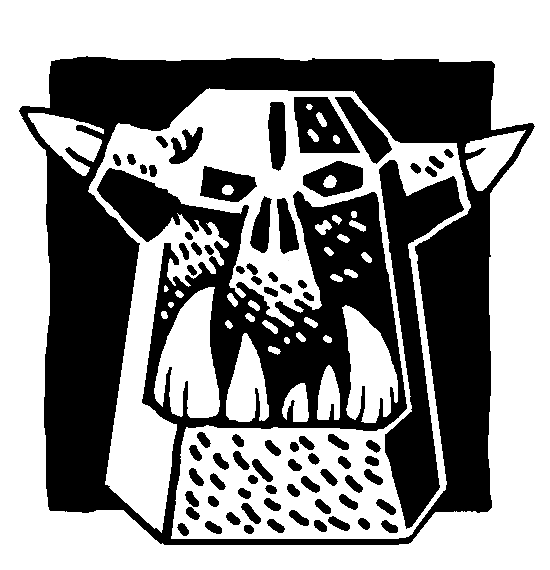
\includegraphics[width=0.8cm]{pics/ironorc.png} &
\largerfontsize\antiquefont\ironorc{} (#1) \tabularnewline
\end{tabular}
\vspace*{-0.2cm}
\end{center}
}

\newcommand{\forkraceFeralOrc}[1]{%
\begin{center}
\begin{tabular}{@{}m{0.8cm}@{\hskip 2pt}l@{}}
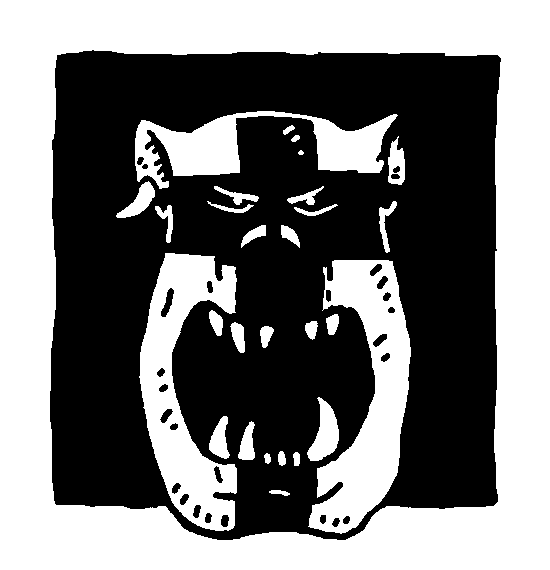
\includegraphics[width=0.8cm]{pics/feralorc.png} &
\largerfontsize\antiquefont\feralorc{} (#1) \tabularnewline
\end{tabular}
\vspace*{-0.2cm}
\end{center}
}

\newcommand{\forkraceCommonGoblin}[1]{%
\begin{center}
\begin{tabular}{@{}m{0.8cm}@{\hskip 2pt}l@{}}
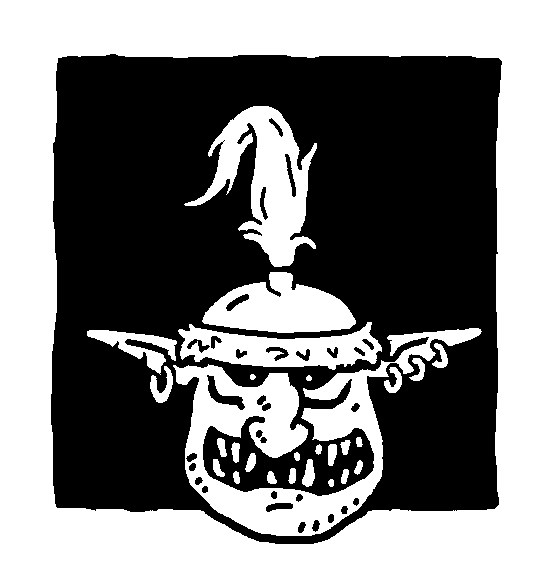
\includegraphics[width=0.8cm]{pics/commongoblin.png} &
\largerfontsize\antiquefont\commongoblin{} (#1) \tabularnewline
\end{tabular}
\vspace*{-0.2cm}
\end{center}
}

\newcommand{\forkraceCaveGoblin}[1]{%
\begin{center}
\begin{tabular}{@{}m{0.8cm}@{\hskip 2pt}l@{}}
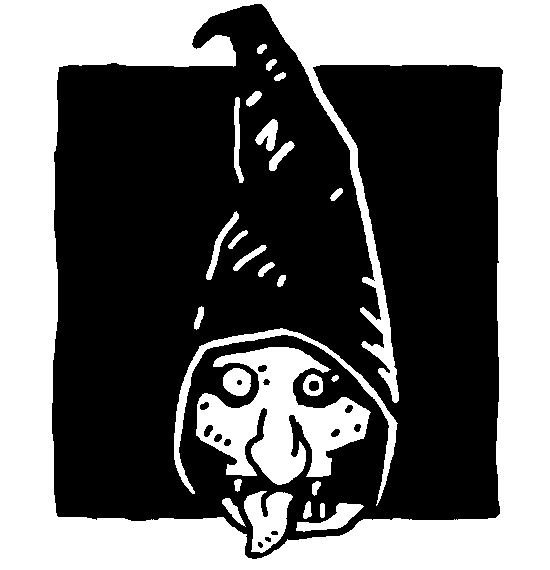
\includegraphics[width=0.8cm]{pics/cavegoblin.png} &
\largerfontsize\antiquefont\cavegoblin{} (#1) \tabularnewline
\end{tabular}
\vspace*{-0.2cm}
\end{center}
}

\newcommand{\forkraceForestGoblin}[1]{%
\begin{center}
\begin{tabular}{@{}m{0.8cm}@{\hskip 2pt}l@{}}
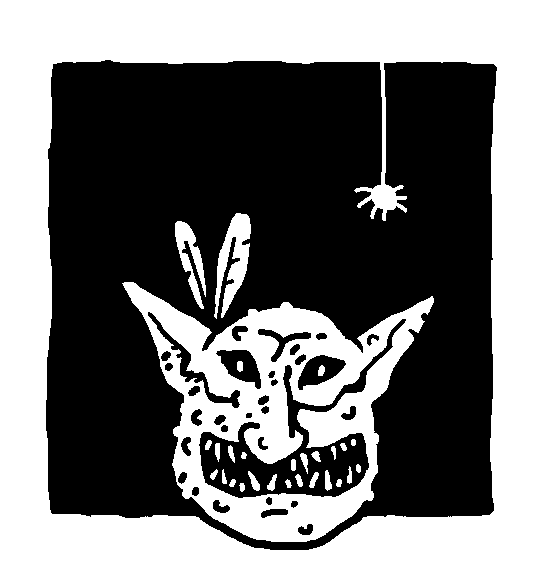
\includegraphics[width=0.8cm]{pics/forestgoblin.png} &
\largerfontsize\antiquefont\forestgoblin{} (#1) \tabularnewline
\end{tabular}
\vspace*{-0.2cm}
\end{center}
}

\newcommand{\labelforinit}{Init.} % \labels@I usually

\newcommand{\profilemodification}[1]{%
\begin{center}\textbf{#1 sur le profil}\end{center}
\vspace{-0.2cm}
}

\newcommand{\closeraceforking}{%
\end{multicols}
\setlength{\columnseprule}{0pt}	
}

% Profile wording

\newcommand{\wyvernnote}{Les \wyverns{} montées par des \orcchiefs{} ont la règle Unique. Cela n'a aucune incidence sur le nombre de \wyverns{} qui peuvent être montées par des \orcwarlords{}.}
\newcommand{\mayexchangeallequipmentforcrossbowandha}{Peut échanger tout son équipement contre une \crossbow{} et une \ha{}}
\newcommand{\maytakeamammothstabber}{L'unité peut prendre un \mammothstabber{}}
\newcommand{\takeshadygits}{Jusqu'à 3 \shadygits{}}
\newcommand{\shadygitlimitation}{Maximum 1 \shadygit{} par tranche de 10 \commongoblins{} dans l'unité.}
\renewcommand{\pershadygit}{/Vengeur}
\newcommand{\madgitlimitation}{Maximum 1 \madgit{} par tranche de 15 \cavegoblins{} dans l'unité.}
\newcommand{\exchangeallweaponsforshieldandshortbow}{Échanger les armes contre un Arc Court et un Bouclier}
\newcommand{\takemadgits}{Jusqu'à 3 \madgits{}}
\renewcommand{\permadgit}{/Fou}
\newcommand{\takenets}{\nets}
\newcommand{\gitnote}{\textbf{Option} pour les unités de \goblins}
\newcommand{\ironorcwarlord}{Seigneur de Guerre \ironorc{}}
\newcommand{\ironorcchief}{Caïd \ironorc{}}
\newcommand{\maytakeanorcoverseer}{Peut prendre un \orcoverseer{}}
\newcommand{\zerotothreechoice}{(Jusqu'à 3)}
\newcommand{\maytakeweblauncher}{Peut prendre un \weblauncher{}}
\newcommand{\spidermothershrineoption}{Si le Cavalier est un Sorcier, peut prendre un \spidermothershrine}

% Profile rules

\newcommand{\netsrule}{%
Au début de chaque Manche de Corps à Corps, choisissez une unité en contact socle à socle avec l'unité possédant des \nets{}. Jetez 1D6.

Sur 2+, la cible subit un malus de -1 en Force (jusqu'à un minimum de 1) jusqu'à la fin du tour de joueur.

Sur un résultat de \result{1}, l'unité qui a utilisé les \nets{} subit le malus à sa place. Une unité ne peut être affectée par des \nets{} qu'une seule fois par Phase.
}

\newcommand{\motherskissrule}{%
Au début de chaque Manche de Corps à Corps, jetez 1D6.

Sur 2+, l'unité gagne des \poisonedattacks{} jusqu'à la fin de la Manche de Corps à Corps.

Sur un résultat de \result{1}, déterminer aléatoirement une unité ennemie en contact socle à socle avec l'unité. Elle gagne des \poisonedattacks{} contre l'unité ayant la règle \motherskiss{} jusqu'à la fin de la Manche de Corps à Corps.
}

\newcommand{\sneakyrule}{%
Les \shadygits{} comptent comme des Champions et sont obligatoirement déployés Cachés dans leur unité. Les \shadygits{} sont automatiquement révélés à la première Manche de Corps à Corps auquel leur unité prend part. Ils ne peuvent pas être révélés plus tôt. Lorsqu'ils sont révélés, les \shadygits{} gagnent +3 en Initiative et la règle \lightningreflexes{} jusqu'à la fin du tour. Les \shadygits{} ne bénéficient ni de Premier entre ses Pairs ni de Meneur de Charge (règles habituelles des Champions).
}

\newcommand{\surpriserule}{%
Les \madgits{} ne sont pas déployés normalement mais cachés dans leur unité. Ce sont des options d'unité, donc ils sont ignorés quand ils sont détruits pour le calcul des Points de Victoire, leur valeur étant déjà incluse dans l'unité de \goblins{} les cachant. Il faut donc détruire cette dernière unité pour gagner leurs Points de Victoire. Avant d'être lâchés hors de leur unité, les \madgits{} ne peuvent pas être affectés par quoi que ce soit, ni avoir d'effet sur la partie. Les \madgits{} détruits ne provoquent pas de tests de Panique. Ils ne comptent pas dans le nombre de figurines de leur unité. Une fois relâchés, ils bougent, agissent et suivent leurs règles spéciales indépendamment comme toute autre unité individuelle.

Ils peuvent être relâchés de deux façons :
\begin{customsubitemize}
\item N'importe quel nombre de \madgits{} peut être relâché quand leur unité déclare comme réaction à une charge Tenir la Position ou Tenir la Position et Tirer.
\item Tous les \madgits{} doivent être relâchés si l'unité les cachant n'est ni en fuite ni engagée au Corps à Corps au début de la Phase de Tir du propriétaire et qu'elle est à moins de \distance{8} d'une unité ennemie.
\end{customsubitemize}

Occupez-vous des \madgits{} l'un après l'autre. Placez le \madgit{} en contact socle à socle avec son unité (il ne lui inflige aucune touche pour ce contact), et choisissez une direction. Déplacez-le de \distance{2D6} dans cette direction. Le \madgit{} suit ensuite ses propres règles pour son déplacement lors des tours suivants.
}

\newcommand{\oiitbitesrule}{%
Aucun Personnage ne peut rejoindre cette unité.
}

\newcommand{\rowsofteethrule}{%
Les \gnashers{} peuvent faire les Attaques de Soutien à la place de leurs Cavaliers.

Les \gnasherdashers{} infligent des Touches d'Impact lorsqu'ils chargent. Au lieu d'infliger une touche par \gnasherdasher{} en charge au contact d'un ennemi, le nombre de Touches d'Impact dépend du nombre de figurines dans l'unité. L'unité inflige 1D3 Touches d'Impact par tranche de 5 \gnasherdashers{}, en arrondissant au supérieur, à une unique unité ennemie en contact.
}

\newcommand{\theyreeverywhererule}{%
Quand une \gnasherherd{} est démoralisée au Corps à Corps, elle est immédiatement retirée du champ de bataille comme perte, et toutes les unités à moins de \distance{6} subissent une touche de Force 5 par tranche de 5 \gnashers{} qui restaient dans la \gnasherherd{}.
}

\newcommand{\orcoverseerrule}{%
La \warmachine{} gagne un servant supplémentaire, de Race \commonorc{}. Elle gagne 1 PV et perd la règle \insignificant{}.

La \warmachine{} peut choisir de perdre 1 PV pour relancer un jet sur la Table des Incidents de Tir.
}

\newcommand{\splattererrule}{%
\textbf{\artilleryweapon} de type \textbf{\catapult{} (\distance{3})}.\newline
\range{12-60}, Force 3 [9], [\multiplewounds{\ordnance}{}].
}

\newcommand{\gitlauncherrule}{%
\textbf{\artilleryweapon} de type \textbf{\catapult{} (\distance{1})}.\newline
\range{12-60}, Force 5, \armourpiercing{2}.

\vspace{5pt}\noindent Après avoir fait dévier le gabarit, vous pouvez le déplacer dans la direction de votre choix sur une distance de \distance{1D6}. Vous ne pouvez cependant pas le déplacer délibérément sur des unités au Corps à Corps ou des unités amies, si cela peut être évité. Une fois la position finale obtenue, au lieu de suivre les règles habituelles des gabarits, toute unité sous le gabarit subit 1D3+1 touches.
}

\newcommand{\pointedsticksrule}{%
Les Touches d'Impact de la \scrapwagon{} bénéficient de \armourpiercing{2}.
}

\newcommand{\pursuitmoderule}{%
Lancez 1D6 supplémentaire pour le \randommovement{} pendant la Phase de Mouvement, et ignorez le dé ayant donné le résultat le plus bas.
}

\newcommand{\smellslikegreenspiritrule}{%
La \scrapwagon{} gagne les règles \distracting{} et \hardtarget{}.
}

\newcommand{\smasherrule}{%
La \scrapwagon{} obtient Force 5.
}

\newcommand{\trollbelchrule}{%
Au lieu d'attaquer normalement au Corps à Corps, un Troll peut choisir de faire une unique Attaque Spéciale de Corps à Corps qui touche automatiquement avec Force 5 et \armourpiercing{6}.
}


\newcommand{\giantattacksrule}{%
Quand un Géant attaque au Corps à Corps, au lieu d'attaquer normalement, choisissez une unité en contact socle à socle à attaquer et lancez 1D6. Déterminez ci-dessous la table à utiliser selon le Type de Troupe de l'unité visée, et trouvez l'attaque correspondant au résultat du dé. Il est important de noter que les Attaques de Géant comptent comme des attaques de Corps à Corps et suivent ainsi normalement les règles affectant ces attaques. Le Géant peut également faire son \stomp{}.
}

\newcommand{\giantattackstable}{%
\setlength{\columnseprule}{0.5pt}
\renewcommand{\columnseprulecolor}{\color{black!30}}
\vspace*{-0.2cm}\begin{multicols}{2}
	\noindent Si l'unité est de type \infantry{}, \warbeast{}, \cavalry{}, \swarm{} ou \warmachine{}  :	
	\renewcommand{\arraystretch}{1.5}	
	\begin{center}\begin{tabular}{cl}
   		\hline
		1 & \bellow{} \tabularnewline
		2 & \jump{} \tabularnewline
		3 & \grab{} \tabularnewline
		4-6 & \swing{} \tabularnewline
		\hline
	\end{tabular}\end{center}
	\vspace*{\fill}
	\columnbreak
	Si l'unité est de type \monstrousinfantry{}, \monstrouscavalry{}, \monstrousbeast{}, \chariot{}, \monster{} ou \riddenmonster{} :
	\begin{center}\begin{tabular}{cl}
		\hline	
		1 & \bellow{} \tabularnewline
		2-3 & \thump{} \tabularnewline
		4-6 & \smashname{} \tabularnewline
		\hline
	\end{tabular}\end{center}
	\vspace*{\fill}
	\renewcommand{\arraystretch}{1.2} % return to default
\end{multicols}
}

\newcommand{\bellowrule}{%
Ni le Géant, ni l'unité sélectionnée ne peuvent faire d'attaques de Corps à Corps pendant cette phase. Les attaques déjà réalisées, incluant celles réalisées simultanément avec cette attaque, ne sont pas concernées. Le camp du Géant gagne automatiquement le combat de 2. Si deux Géants opposés, ou plus, \og{} Hurlent \fg{}, le combat est un match nul.
}

\newcommand{\jumprule}{%
L'unité sélectionnée subit 1D6 touches de la Force du Géant. Le Géant doit faire un test de Terrain Dangereux (1).
}

\newcommand{\grabrule}{%
Choisissez une figurine dans l'unité sélectionnée et en contact socle à socle avec le Géant. Cette figurine doit faire un test de Force et un test de Capacité de Combat. Pour chaque test raté, la figurine subit une touche de la Force du Géant et suivant la règle spéciale \multiplewounds{1D3}{}.
}

\newcommand{\swingrule}{%
Le Géant fait 2D6 attaques sur l'unité choisie.
}

\newcommand{\thumprule}{%
Choisissez une figurine en contact socle à socle avec le Géant dans l'unité sélectionnée. Cette figurine doit faire un test d'Initiative. Si elle échoue, la figurine subit 2D6 blessures avec \armourpiercing{6}.
}

\newcommand{\smashrule}{%
Choisissez une figurine en contact socle à socle avec le Géant dans l'unité sélectionnée. Cette figurine subit une blessure avec \armourpiercing{6}. Si la figurine n'a pas encore attaqué, elle ne peut plus le faire au cours de cette manche. Si la figurine a déjà réalisé ses attaques, elle ne pourra pas attaquer au cours du tour de  joueur à venir.
}

\newcommand{\ballistarule}{%
\textbf{\artilleryweapon} de type \textbf{\boltthrower}.

\range{48}, Force 6, \multiplewounds{1D3}{}, \armourpiercing{6}.
}

\newcommand{\lookatemgorule}{%
Le \gnasherwreckingteam{} gagne la règle \runningamok{} quand il touche une unité pour la première fois de la partie.
}

\newcommand{\weblauncherrule}{%
\textbf{\artilleryweapon} de type \textbf{\catapult{} (\distance{3})}.

\range{6-36}, Force 3.

Les unités touchées souffrent d'un malus de -1D3 à l'Initiative. Les Terrains Dangereux (1) comptent pour eux comme des Terrains Dangereux (2), et tous les autres éléments de décor, Terrain Découvert compris, comptent pour eux comme des Terrains Dangereux (1). Ces effets durent jusqu'à la fin du prochain Tour de Joueur. Les effets de différents \weblaunchers{} ne s'additionnent pas.
}

\newcommand{\smashemflatrule}{%
Si l'\greatgreenidol{} est engagée au Corps à Corps, toutes les unités amies à moins de \distance{8} peuvent gagner la règle \devastatingcharge{} ou un bonus de +1 pour blesser. Chaque unité choisit quel bonus utiliser au début de chaque Round de Corps à Corps.
}

\newcommand{\iconofthewaaarghrule}{%
Une \greatgreenidol{} bénéficie des avantages de la \waaargh{} comme si elle appartenait à une \greenhiderace.
}

\newcommand{\bouncersrule}{%
Ne peut rejoindre que des unités de \cavegnashers{} et de \gnasherdashers{}, ignorez pour cela les restrictions des règles \skirmishers{} et \oiitbites{}.
}

\newcommand{\spidermothershrinerule}{%
Le Sorcier gagne la règle \pathmaster{}. Toutes les figurines amies avec la capacité de \channel{} à moins de \distance{12} ajoutent +2 au lieu de +1 à la tentative de \channel{}.
}

% QRS note

\newcommand{\QRSnote}{%
\noindent$^{1}$ Un \ironorc{} gagne +1 CC.

\noindent$^{2}$ Un \cavegoblin{} gagne +1 I.

\noindent$^{3}$ Un \cavegoblin{} gagne +1 I et -1 Cd.

\noindent$^{4}$ Un membre d'équipage de moins quand il sert de monture.
}




\begin{document}

\newgeometry{margin=1in}

% Table options
\arrayrulecolor{black!30}
\setlength{\arrayrulewidth}{2pt}
\renewcommand{\arraystretch}{1.2}

\begin{titlepage}
\begin{center}

\ifdef{\booktitle}{}{\newcommand{\booktitle}{Missing title}}
\ifdef{\version}{}{\newcommand{\version}{Missing version}}

{\antiquefont\fontsize{40}{48}\selectfont\noindent\labels@fantasybattles

\labels@NinthAge}

\vspace*{0.5cm}
\ifdef{\booklogo}{%
\includegraphics[height=10cm]{\booklogo}%
}{%

\includegraphics[height=10cm]{../Layout/pics/logo_9th.png}%
}

\vspace*{-1cm}
{\antiquefont\fontsize{50}{60}\selectfont \booktitle
\vspace{0.4cm}

\fontsize{14}{16.8}\selectfont \labels@armyrules{}

Beta v\version{} - \today{}}

\ifdef{\frenchversion}{{\fontsize{14}{16.8}\selectfont \vspace{0.2cm}\noindent\texttt{VF \frenchversion}}}{}
\vfill

\begin{tabular}{@{}m{2cm}@{\hskip 20pt}m{13cm}@{}}

\includegraphics[width=2cm]{../Layout/pics/seal_9th.png} &
{\fontsize{10}{12}\selectfont \textcolor{black!50}{\noindent\labels@frontpagecredits}}

\ifdef{\frontpageaddstuff}{{\fontsize{10}{12}\selectfont \noindent\textcolor{black!50}{\frontpageaddstuff}}}{}

\vspace*{10pt}
\noindent{\fontsize{10}{12}\selectfont \textcolor{black!50}{\labels@license}}
\tabularnewline
\end{tabular}


\end{center}

\newpage

\thispagestyle{empty}

{\fontsize{10}{12}\selectfont

\ifdef{\labels@introduction}{\labels@introduction}{\vphantom{1pt}}
\vfill

\noindent\newrule{\labels@rulechanges}

\bigskip
\noindent \labels@latexcredit
}


\end{titlepage}

\restoregeometry

\startarmyspecialrules

\armyspecialruleentry{\greenhideraces}

Certaines figurines de l'armée disposent de règles spéciales qui correspondent à leur race.

\newcommand{\logosize}{3cm}
\begin{multicols}{3}\raggedcolumns

\begin{center}

\includegraphics[width=\logosize]{pics/commonorc.png}
\vspace*{-1cm}\subsubtitle{\commonorc}

\unruly{}, \borntofight{}
\end{center}

\columnbreak

\begin{center}
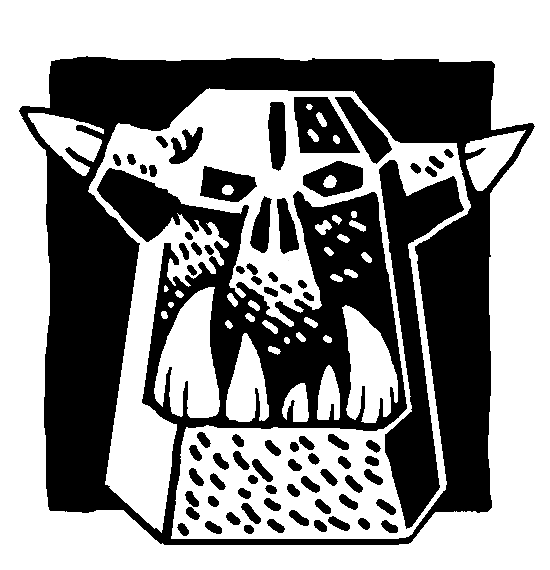
\includegraphics[width=\logosize]{pics/ironorc.png}
\vspace*{-1cm}\subsubtitle{\ironorc}

\immunetopsychology{}, \weaponmaster{}, \borntofight{}
\end{center}

\columnbreak

\begin{center}
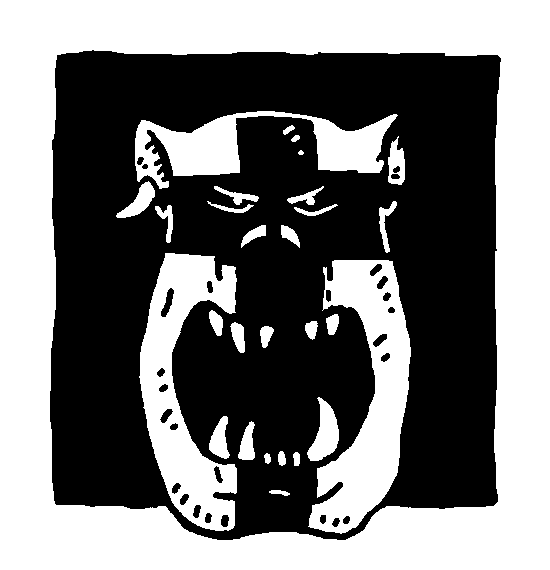
\includegraphics[width=\logosize]{pics/feralorc.png}
\vspace*{-1cm}\subsubtitle{\feralorc}

\frenzy{}, \unruly{}, \borntofight{}, \wardsave{6}
\end{center}

\end{multicols}

\begin{multicols}{3}\raggedcolumns

\begin{center}
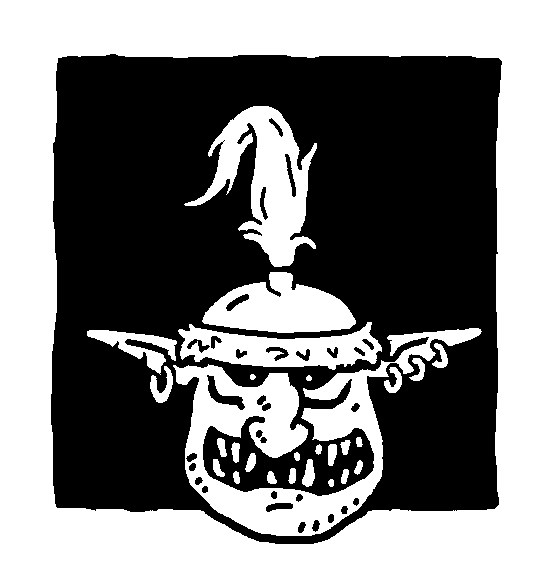
\includegraphics[width=\logosize]{pics/commongoblin.png}
\vspace*{-1cm}\subsubtitle{\commongoblin}

\unruly{}, \insignificant{}
\end{center}

\columnbreak

\begin{center}
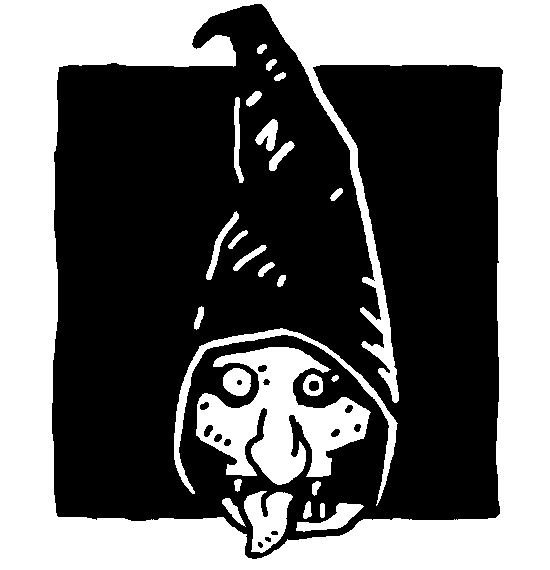
\includegraphics[width=\logosize]{pics/cavegoblin.png}
\vspace*{-1cm}\subsubtitle{\cavegoblin}

\hatred{} (Livre d'Armée : Forteresses Naines), \unruly{}, \insignificant{}
\end{center}

\columnbreak

\begin{center}
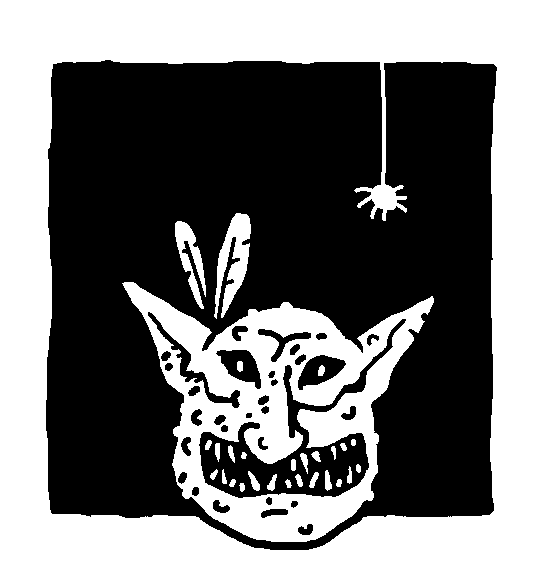
\includegraphics[width=\logosize]{pics/forestgoblin.png}
\vspace*{-1cm}\subsubtitle{\forestgoblin}

\strider{\forest}, \unruly{}, \insignificant{}
\end{center}

\end{multicols}

\armyspecialruleentry{\unruly}

Les figurines avec cette règle ont un malus de -1 en Commandement pour les tests de \frenzy{} et pour se réfréner de poursuivre. Si elles sont en formation de Horde, jetez trois dés pour les tests de Panique et ignorez le dé ayant donné le plus grand résultat.

\armyspecialruleentry{\borntofight}

L'élément de figurine gagne +1 en Force lors de la première Manche de Corps à Corps.


\begin{multicols}{2}\raggedcolumns
\setlength{\columnseprule}{1pt}
\renewcommand{\columnseprulecolor}{\color{black!30}}
\armyspecialruleentry{\waaargh}

Une fois par partie, le Général peut déclarer une \waaargh{} au début du tour de n'importe quel joueur. Toutes les figurines ayant des éléments appartenant à une Race de Peaux Vertes gagnent +1 en Mouvement et la règle \swiftstride{} jusqu'à la fin du Tour de Joueur.

\columnbreak
\armyspecialruleentry{\greentide}

Une fois par partie, le Général peut déclarer une \greentide{} au début du tour de n'importe quel joueur. Tous les éléments de figurine appartenant à une Race Peau Verte de \goblins{} gagnent la règle \fightinextrarank{} jusqu'à la fin du Tour de Joueur suivant.

\end{multicols}

\armyspecialruleentry{\venomousfangs}

Désignez une des attaques de Corps à Corps de l'élément de figurine avant de lancer les dés pour toucher. Cette attaque gagne \multiplewounds{\ordnance}{}.

\armyspecialruleentry{\shambolic{X}}

L'unité a \randommovement{X}. Elle gagne la règle \immunetopsychology{} et ne peut pas être rejointe par des Personnages. Si elle obtient le même résultat sur tous les dés lors de son jet de \randommovement{}, elle subit 1D3 blessures sans sauvegarde d'aucune sorte, puis se déplace de cette distance dans une direction aléatoire.

Si elle arrive au contact d'un élément de décor autre qu'un Terrain Découvert ou une Colline, si elle arrive au contact d'un bord de table ou si elle s'arrête à \distance{1} d'un Terrain Infranchissable, elle doit faire un test de Terrain Dangereux (2).

\armyspecialruleentry{\runningamok}

Une unité avec \shambolic{} et \runningamok{} se déplace toujours dans une direction aléatoire lors de son \randommovement{}.

\armyspecialruleentry{\ricochet{X}}

Les figurines avec \ricochet{} ignorent l'écart d'\distance{1} avec les autres unités. Si une figurine avec cette règle touche une autre unité, amie ou ennemie, au lieu de charger, elle continue son mouvement dans la même direction jusqu'à respecter la règle des \distance{1} d'écart entre unités et avoir parcouru au moins sa distance de mouvement. Si cela devait amener la figurine au contact, ou à moins d'\distance{1} d'une autre unité, elle continue à se déplacer dans la même direction jusqu'à pouvoir se trouver à plus d'\distance{1} de toute autre unité. Si elle se retrouve alors à moins d'\distance{1} d'un Terrain Infranchissable ou en dehors du champ de bataille, retirez-la comme perte.

Toute unité traversée durant le déplacement jusqu'à la distance obtenue sur les dés pour le \randommovement{} est touchée par une Attaque Spéciale à distance. Les unités touchées subissent X touches, X étant la valeur entre les parenthèses. Les unités engagées dans un même Corps à Corps ne comptent que comme une seule unité pour la détermination des touches. Le joueur possédant la figurine avec \ricochet{} répartit les touches infligées entre les unités en combat aussi équitablement que possible, puis applique les règles normales de distribution des touches dans chaque unité.

Il n'est pas possible de charger une figurine avec \ricochet{}, mais une unité peut charger, fuir, poursuivre ou se déplacer à travers elle. L'unité subit alors X+1D6 touches, puis la figurine avec \ricochet{} est retirée du champ de bataille en tant que perte.

Toutes les touches sont infligées avec la Force non modifiée de la figurine et ont \armourpiercing{1}.

\vspace{1cm}
\begin{center}
\begin{tabular}{@{}m{9.5cm}@{\hskip 20pt}m{7.5cm}@{}}
\def\svgwidth{9.5cm}
\input{pics/ricochet.pdf_tex}
&
\textbf{a)} La figurine avec \ricochet{} ne peut pas être placée à plus d'\distance{1} derrière l'unité rose car l'unité verte est trop proche. Elle est donc déplacée à travers les deux unités en suivant la direction initiale. Seule l'unité rose subit les touches de Ricochet car l'unité verte se situe au delà de la distance de mouvement obtenue aux dés.

\vspace{10pt}\textbf{b)} Après avoir été déplacée à travers les unités, la figurine avec \ricochet{} arrive à moins d'\distance{1} d'un Terrain Infranchissable et est donc retiré comme perte. Elle a traversé au moins une unité engagée au Corps à Corps, infligeant donc X touches en tout, qui doivent être distribuées équitablement entre toutes les unités en combat.
\tabularnewline
\end{tabular}
\end{center}

\closearmyspecialrules



\newpage
\startarmyarmoury

\startitemlistonecol

\listitemonecol{\powershroom} Une seule utilisation. Avant de jeter les dés pour lancer un sort qui ne vient pas d'un Objet de Sort, le porteur peut décider d'utiliser un \powershroom{}. Toute tentative de dissipation de ce sort voit sa valeur réduite de 1D3. Si un \result{1} naturel est obtenu, le Sorcier utilisant le \powershroom{} subit une touche avec la règle Attaques Toxiques.

\listitemonecol{\mammothstabber} Si l'unité possède au moins un Rang Complet, elle gagne 1D3 \impacthits{} de Force 5 avec \multiplewounds{\ordnance}{\largetarget}.

\enditemlistonecol

\closearmyarmoury


\renewcommand{\startarmymagicalitems}{\vspace{1cm}\largefontsize\bigtitle{\labels@magicalitems}\begin{multicols}{2}\raggedcolumns}

\startarmymagicalitems

\armymagicalweapons

\startpricelist

\pricelistitem{Hache de l'Aporcalypse}{65/45}Type : \hw{}. Le porteur gagne +1D3 en Force et +1D3 Attaques. Ces bonus sont déterminés et prennent effet au palier d'Initiative auquel le porteur attaque avec cette arme.

\pricelistitem{Arc Zap de Maza}{30} \goblin{} uniquement.

Type : Arc. \range{24}, Force 3, \lightningattacks{}, \multipleshots{3}. L'unité du porteur gagne la règle spéciale \quicktofire{}.

\pricelistitem{Dague de Sournois}{15}Type : \hw{}. Les attaques portées avec cette arme ont \armourpiercing{1}. Si le porteur attaque une unité ennemie de flanc ou de dos, ses attaques avec cette arme gagnent +2 en Force.

\endpricelist

\armymagicalarmour

\startpricelist

\pricelistitem{Couronne du Roi des Cavernes}{40}\goblin{} uniquement. Ne peut pas être pris par une \largetarget{}.

Type : Aucun. Sauvegarde d'Armure de 6+. Le porteur ne peut rejoindre ou être rejoint que par une unité dont toutes les figurines ont au moins un élément qui partage la même \greenhiderace{} que lui. L'unité du porteur gagne alors la règle \vanguard{} et peut se déplacer après un ralliement, mais elle ne peut alors ni tirer, ni faire de Marche Forcée. De plus, la portée de la \inspiringpresence{} ou de \holdyourground{} du porteur est augmentée de \distance{6}.

\pricelistitem{Plaques de Tuktek}{35}Type : \ha{}. Le porteur gagne +1 en Endurance et la figurine du porteur gagne 1D3 \impacthits{}.

\endpricelist

\armytalismans

\startpricelist

\pricelistitem{Chapardeur de Défense}{15}\goblin{} uniquement.

Si le porteur subit une blessure, il peut utiliser la Sauvegarde d'Armure, la \wardsave{}, la \regeneration{} et la \magicresistance{} de la figurine lui ayant infligé cette blessure.

\endpricelist

\armyenchanteditems

\startpricelist

\pricelistitem{Patte de Sanglier}{20}Figurine montée uniquement.

Toutes les figurines alliées de type Cavalerie à moins de \distance{18} du porteur peuvent relancer leurs tests de Terrain Dangereux.

\pricelistitem{Peintures Waaargh!}{15}\feralorc{} uniquement.

Le porteur gagne la \frenzy{} et ne peut jamais la perdre. De plus, tous les \feralorcs{} de l'unité du porteur gagnent la \frenzy{} tant que ce dernier est dans l'unité. Enfin, l'unité gagne la règle \swiftstride{} pour les mouvements de Poursuite et de Charge Irrésistible.

\endpricelist

\armymagicalbanners

\startpricelist

\pricelistitem{Totem de Mikinok}{40}Les autres Objets Magiques dans l'unité du porteur ainsi que dans les unités amies ou ennemies en contact avec l'unité du porteur n'ont plus d'effet et redeviennent des objets ordinaires. Cet effet dure tant que les unités restent en contact.

\pricelistitem{Icône de Blindage}{25}L'unité du porteur gagne une \wardsave{5} contre les Attaques de Tir.

\endpricelist

\closearmymagicalitems





%%% START OF THE ARMYLIST - Translators shouldn't have to edit it %%%

%%% v0.99.2

\armylist

\lordstitle

\showunit{
	name={\orcwarlord},
	QRSname={\orcwarlordinQRS{}$^{1}$},
	cost={120},
	profile={ < 4 6 3 5 5 3 4 4 9},
	type=\infantry{},
	basesize=25x25,
	unitsize=1,
	options={
		\magicalitemsallowance{}=\upto{}<100,
		\maygain{} \waaargh{} \only{\general}=20,
		\anyofthefollowing{
			\shield{}=5,
			\pw{}=5,
			\gw{}=15,
			\lance{}=15,
		},
	},
	additional={%
		\startraceforking{3}%
			\forkraceCommonOrc{\free}%
		
			\def\temparmour{\la{}}%
			\armour{\temparmour}

			\def\tempoptions{\ha{}=12,}%
			\vspace*{0.1cm}\options{\tempoptions}

			\def\tempmounts{\warboar{}=20,\orcboarchariot{}=30,\wyvern{}=120}%
			\mounts{\tempmounts}

		\vspace*{\fill}
		\columnbreak
			\forkraceIronOrc{\pts{20}}%

			\profilemodification{+1 \labels@WS{}}

			\def\temparmour{\ha{}}%
			\armour{\temparmour}

			\def\tempoptions{\platearmour{}=20,}%
			\vspace*{0.1cm}\options{\tempoptions}

			\def\tempmounts{\warboar{}=20,\orcboarchariot{}=30,\wyvern{}=120}%
			\mounts{\tempmounts}

		\vspace*{\fill}
		\columnbreak
			\forkraceFeralOrc{\pts{15}}%

			\def\tempmounts{\warboar{}=10,\wyvern{}=105}%
			\mounts{\tempmounts}

		\vspace*{\fill}
		\closeraceforking{}%
	},
}

\showunit{
	name={\orcbigshaman},
	cost={175},
	profile={ < 4 3 3 4 5 3 2 1 8},
	type=\infantry{},
	basesize=25x25,
	unitsize=1,
	magiclevel=3,
	magicpaths={\thebiggreengods{},\wilderness{}},
	options={
		\magicalitemsallowance{}=\upto{}<100,
		\magiclevel{4}=30,
	},
	additional={%
		\startraceforking{2}%
			\forkraceCommonOrc{\free}%

			\def\tempmounts{\warboar{}=20,\orcboarchariot{}=20,\wyvern{}=120}%
			\mounts{\tempmounts}

		\vspace*{\fill}
		\columnbreak
			\forkraceFeralOrc{\pts{5}}%

			\def\tempmounts{\warboar{}=20,\wyvern{}=120}%
			\mounts{\tempmounts}

		\vspace*{\fill}
		\closeraceforking{}%
	},
}

\showunit{
	name={\goblinking},
	QRSname={\goblinking{}$^{2}$},
	cost={60},
	profile={ < 4 5 4 4 4 3 4 4 8},
	type=\infantry{},
	basesize=20x20,
	unitsize=1,
	armour={\la},
	options={
		\magicalitemsallowance{}=\upto{}<100,
		\maygain{} \greentide{} \only{\general}=10,
		\anyofthefollowing{
			\shield{}=5,
			\ha{}=8,
		},
		\maytakeashortbow{}=5,
		\weapononechoice{
			\pw{}=5,
			\gw{}=15,
			\lance{}=15,
		},
	},
	additional={%
		\startraceforking{3}%
			\forkraceCommonGoblin{\free}%

			\def\tempmounts{\wolf{}=15,\goblinwolfchariot{}=25}%
			\mounts{\tempmounts}

		\vspace*{\fill}		
		\columnbreak
			\forkraceCaveGoblin{\pts{5}}%

			\profilemodification{+1 \labelforinit{}}

			\def\tempmounts{\cavegnasher{}=20}%
			\mounts{\tempmounts}

		\vspace*{\fill}
		\columnbreak
			\forkraceForestGoblin{\free}%

			\def\tempoptions{\poisonedattacks{}=10}
			\options{\tempoptions}
			
			\def\tempmounts{\scuttlerspider{}=20,\huntsmenspider{}=20,\gargantula{}=250}%
			\mounts{\tempmounts}

		\vspace*{\fill}
		\closeraceforking{}%
	},
}

\showunit{
	name={\goblinbigshaman},
	QRSname={\goblinbigshaman{}$^{3}$},
	cost={170},
	profile={ < 4 2 3 3 4 3 2 1 7},
	type=\infantry{},
	basesize=20x20,
	unitsize=1,
	magiclevel=3,
	magicpaths={\thelittlegreengods{},\shadows{}},
	options={
		\magicalitemsallowance{}=\upto{}<100,
		\magiclevel{4}=30,
	},
	additional={%
		\startraceforking{3}%
			\forkraceCommonGoblin{\free}%

			\def\tempmounts{\wolf{}=15,\goblinwolfchariot{}=20}%
			\mounts{\tempmounts}

		\vspace*{\fill}		
		\columnbreak
			\forkraceCaveGoblin{\free}%

			\profilemodification{+1 \labelforinit{} \wordand{} -1 \labels@Ld{}}

			\def\tempoptions{\powershrooms{}=15}
			\options{\tempoptions}

		\vspace*{\fill}
		\columnbreak
			\forkraceForestGoblin{\free}%
			
			\def\tempmounts{\scuttlerspider{}=15,\gargantula{}=250}%
			\mounts{\tempmounts}

		\vspace*{\fill}
		\closeraceforking{}%
	},
}

\heroestitle

\showunit{
	name={\orcchief},
	QRSname={\orcchief{}$^{1}$},
	cost={50},
	profile={ < 4 5 3 4 5 2 3 3 8},
	type=\infantry{},
	basesize=25x25,
	unitsize=1,
	options={
		\bsboption{}=25,
		\magicalitemsallowance{}=\upto{}<50,
		\maygain{} \waaargh{} \only{\general}=10,
		\anyofthefollowing{
			\shield{}=5,
			\pw{}=5,
			\gw{}=10,
			\lance{}=10,
		},
	},
	additional={%
		\startraceforking{3}%
			\forkraceCommonOrc{\free}%
		
			\def\temparmour{\la{}}%
			\armour{\temparmour}

			\def\tempoptions{\ha{}=5,}%
			\vspace*{0.1cm}\options{\tempoptions}

			\def\tempmounts{\warboar{}=15,\orcboarchariot{}=60,\wyvern{}=150}%
			\mounts{\tempmounts}

		\vspace*{\fill}		
		\columnbreak
			\forkraceIronOrc{\pts{10}}%

			\profilemodification{+1 \labels@WS{}}

			\def\temparmour{\ha{}}%
			\armour{\temparmour}

			\def\tempoptions{\platearmour{}=15,}%
			\vspace*{0.1cm}\options{\tempoptions}

			\def\tempmounts{\warboar{}=15,\wyvern{}=150}%
			\mounts{\tempmounts}

		\vspace*{\fill}
		\columnbreak
			\forkraceFeralOrc{\pts{5}}%

			\def\tempmounts{\warboar{}=15,\wyvern{}=150}%
			\mounts{\tempmounts}

		\vspace*{\fill}
		\closeraceforking{}%
	},
}

\showunit{
	name={\orcshaman},
	cost={65},
	profile={ < 4 3 3 3 4 2 2 1 7},
	type=\infantry{},
	basesize=25x25,
	unitsize=1,
	magiclevel=1,
	magicpaths={\thebiggreengods{},\wilderness{}},
	options={
		\magicalitemsallowance{}=\upto{}<50,
		\magiclevel{2}=25,
	},
	additional={%
		\startraceforking{2}%
			\forkraceCommonOrc{\free}%

			\def\tempmounts{\warboar{}=15,\orcboarchariot{}=50}%
			\mounts{\tempmounts}

		\vspace*{\fill}
		\columnbreak
			\forkraceFeralOrc{\pts{5}}%

			\def\tempmounts{\warboar{}=15,}%
			\mounts{\tempmounts}

		\vspace*{\fill}
		\closeraceforking{}%
	},
}

\showunit{
	name={\goblinchief},
	QRSname={\goblinchief{}$^{3}$},
	cost={35},
	profile={ < 4 4 4 4 4 2 3 3 7},
	type=\infantry{},
	basesize=20x20,
	unitsize=1,
	armour={\la},
	options={
		\bsboption{}=25,
		\magicalitemsallowance{}=\upto{}<50,
		\maygain{} \greentide{} \only{\general}=20,
		\maytakeashield{}=\free{},
		\maytakeashortbow{}=3,
		\weapononechoice{
			\pw{}=3,
			\lightlance{}=3,
			\gw{}=6,
			\lance{}=6,
		},
	},
	additional={%
		\startraceforking{3}%
			\forkraceCommonGoblin{\free}%

			\def\tempoptions{\ha{}=5,}%
			\options{\tempoptions}
			
			\def\tempmounts{\wolf{}=20,\goblinwolfchariot{}=45}%
			\mounts{\tempmounts}

		\vspace*{\fill}		
		\columnbreak
			\forkraceCaveGoblin{\free}%

			\profilemodification{+1 \labelforinit{} \wordand{} -1 \labels@Ld{}}

			\def\tempmounts{\cavegnasher{}=35}%
			\mounts{\tempmounts}

		\vspace*{\fill}
		\columnbreak
			\forkraceForestGoblin{\free}%

			\def\tempoptions{\poisonedattacks{}=5}
			\options{\tempoptions}
			
			\def\tempmounts{\scuttlerspider{}=15,\huntsmenspider{}=25}%
			\mounts{\tempmounts}

		\vspace*{\fill}
		\closeraceforking{}%
	},
}

\showunit{
	name={\goblinshaman},
	QRSname={\goblinshaman{}$^{3}$},
	cost={60},
	profile={ < 4 2 3 3 3 2 2 1 6},
	type=\infantry{},
	basesize=20x20,
	unitsize=1,
	magiclevel=1,
	magicpaths={\thelittlegreengods{}},
	options={
		\magicalitemsallowance{}=\upto{}<50,
		\magiclevel{2}=25,
	},
	additional={%
		\startraceforking{3}%
			\forkraceCommonGoblin{\free}%

			\def\tempmounts{\wolf{}=15,\goblinwolfchariot{}=40}%
			\mounts{\tempmounts}
	
		\vspace*{\fill}	
		\columnbreak
			\forkraceCaveGoblin{\free}%

			\profilemodification{+1 \labelforinit{} \wordand{} -1 \labels@Ld{}}

			\def\tempoptions{\powershrooms{}=15}
			\options{\tempoptions}

		\vspace*{\fill}
		\columnbreak
			\forkraceForestGoblin{\free}%
			
			\def\tempmounts{\scuttlerspider{}=15}%
			\mounts{\tempmounts}

		\vspace*{\fill}
		\closeraceforking{}%
	},
}

\coreunitstitle

\showunit{
	name={\orcs},
	cost={90},
	profile={< 4 3 3 3 4 1 2 1 7},
	type=\infantry{},
	basesize=25x25,
	unitsize=20,
	maxmodels=50,
	costpermodel=6,
	options={
		\anyofthefollowing{
			\shield{}=\permodel{}<1,
			\bow{}=\permodel{}<1,
			\pw{}=\permodel{}<1,
			\spear{}=\permodel{}<1,
		},
	},
	commandgroup={champion=10, musician=10, banner=10, veteranstandardbearer=yessir},
	additional={%
		\startraceforking{2}%
			\forkraceCommonOrc{\free}%

			\def\temparmour{\la}%
			\armour{\temparmour}%
			
			\def\tempoptions{\mayexchangeallequipmentforcrossbowandha{}=\permodel{}<4,}%
			\vspace*{0.1cm}\options{\tempoptions}%

		\vspace*{\fill}
		\columnbreak
			\forkraceFeralOrc{\pts{2}\permodel}%

			\def\tempoptions{\maytakeamammothstabber{}=15,}%
			\options{\tempoptions}%

		\vspace*{\fill}
		\closeraceforking{}%
	},
}

\showunit{
	name={\orceadbashers{} (\oneofakind)},
	cost={70},
	profile={< 4 4 3 4 4 1 2 1 7},
	type=\infantry{},
	basesize=25x25,
	unitsize=10,
	maxmodels=40,
	costpermodel=9,
	commandgroup={champion=10, musician=10, banner=10, veteranstandardbearer=yessir},
	options={%
		\anyofthefollowing{
			\shield{}=\permodel{}<1,
			\pw{}=\permodel{}<1,
			\spear{}=\permodel{}<1,
		},
	},
	additional={%
		\startraceforking{2}%
			\forkraceCommonOrc{\free}%

			\def\temparmour{\la}%
			\armour{\temparmour}%

		\vspace*{\fill}
		\columnbreak
			\forkraceFeralOrc{\pts{1}\permodel}%

			\def\tempoptions{%
				\maytakeamammothstabber{}=15,
			}%
			\options{\tempoptions}%

		\vspace*{\fill}
		\closeraceforking{}%
	},
}

\showunit{
	name={\goblins},
	QRSname={\goblins{}$^{3}$},
	cost={60},
	profile={ < 4 2 3 3 3 1 2 1 6},
	type=\infantry{},
	basesize=20x20,
	unitsize=20,
	maxmodels=60,
	costpermodel=3,
	options={
		\maytakeoneofthefollowing{
			\shortbow{}=\free{},
			\shield{}=\permodel{}<1,
			\spear{} \&{} \shield{}=\permodel{}<1,
		},
	},
	commandgroup={champion=10, musician=10, banner=10, veteranstandardbearer=yessir},
	additional={%
		\startraceforking{3}%
			\forkraceCommonGoblin{\free}%

			\def\temparmour{\la}
			\armour{\temparmour}
			
			\def\tempoptions{%
				\takeshadygits{}\dotfill{}=\pershadygit{}<15,
				\exchangeallweaponsforshieldandshortbow{}=\permodel{}<1,	
			}%
			\vspace*{0.1cm}\options{\tempoptions}

		\vspace*{\fill}		
		\columnbreak
			\forkraceCaveGoblin{\free}%

			\profilemodification{+1 \labelforinit{} \wordand{} -1 \labels@Ld{}}

			\def\tempoptions{%
				\takemadgits{}=\permadgit{}<30,
				\takenets{}=\permodel{}<1,	
			}%
			\options{\tempoptions}

		\vspace*{\fill}
		\columnbreak
			\forkraceForestGoblin{\free}%

			\def\tempoptions{%
				\throwingweapons{}=\permodel{}<1,
				\motherskiss{}=\permodel{}<1,
				\skirmishers{} \ifNmodelsorless{20}\dotfill{}=\permodel{}<1,
			}
			\options{\tempoptions}

		\vspace*{\fill}
		\closeraceforking{}%
		
		\def\tempunitrules{%
			\unitrule{\nets}{\netsrule}
			\unitrule{\motherskiss}{\motherskissrule}
		}
		\vspace*{0.1cm}\unitrules{\tempunitrules}
	},
}

\showunit{
	name={\shadygit},
	profile={ < 4 4 3 3 3 1 3 2 6},
	cost={15},
	type=\infantry{},
	basesize=20x20,
	unitsize=SPECIAL-\gitnote{},
	greenhiderace={\commongoblin},
	weapons={\pw},
	armour={\la},
	specialrules={\lethalstrike{},\sneaky{}},
	additional={%
		\def\tempunitrules{%
			\unitrule{\sneaky}{\sneakyrule}
		}
		\unitrules{\tempunitrules}		
	},
}

\showunit{
	name={\madgit},
	profile={ < \starsymbol{} - - 5 3 1 3 1 5},
	cost={30},
	type=\infantry{},
	basesize=25,
	unitsize=SPECIAL-\gitnote{},
	greenhiderace={\cavegoblin},
	specialrules={\shambolic{2D6},\runningamok{},\ricochet{1D6},\hardtarget{},\surprise{}},
	additional={%
		\def\tempunitrules{%
			\unitrule{\surprise}{\surpriserule}
		}
		\vspace*{0.1cm}\unitrules{\tempunitrules}		
	},
}

\showunit{
	name={\goblinraiders},
	cost={60},
	profile={
		\rider{}< 4 2 3 3 3 1 2 1 6,
		[\wolf{}]< 9 3 - 3 3 1 3 1 3,
		[\scuttlerspider{}]< 7 3 - 3 3 1 4 1 2,
	},
	type=\cavalry{},
	basesize=25x50,
	unitsize=5,
	maxmodels=20,
	costpermodel=8,
	specialrules={\fastcavalry},
	options={
		\musttakeoneormoreofthefollowing{
			\shield{}=\permodel{}<1,
			\lightlance{}=\permodel{}<1,
			\shortbow{}=\permodel{}<1,
			\throwingweapons{} \only{\forestgoblin}=\permodel{}<1,
		},
	},
	commandgroup={champion=10, musician=10, banner=10},
	additional={%
		\startraceforkingrider{2}%
			\forkraceCommonGoblin{\free}%

			\vspace*{-0.3cm}{\setlength{\parskip}{0.3cm}
			\def\temparmour{\la{},\mountsprotection{6}}
			\armour{\temparmour}
			
			\noindent\unitentryformat{\labels@mount\spacebeforecolon{}:}\newline\wolf{}.
			}

		\vspace*{\fill}
		\columnbreak
			\forkraceForestGoblin{\free}%

			\vspace*{-0.3cm}{\setlength{\parskip}{0.3cm}
			\def\temparmour{\mountsprotection{6}}
			\armour{\temparmour}

			\def\tempspecialrules{\scout{},\strider{},\poisonedattacks{} \only{\scuttlerspider}}
			\specialrules{\tempspecialrules}
			
			\noindent\unitentryformat{\labels@mount\spacebeforecolon{}:}\newline\scuttlerspider{}.
			}

		\vspace*{\fill}			
		\closeraceforking{}%
	},
}

\showunit{
	name={\orcboarriders},
	cost={70},
	profile={%
		\rider{}< 4 3 3 3 4 1 2 1 7,
		\warboar{}< 7 3 - 3 3 1 3 1 3,
	},
	type=\cavalry{},
	basesize=25x50,
	unitsize=5,
	maxmodels=15,
	costpermodel=13,
	weapons={\lightlance},
	specialrules={\thunderouscharge{} \only{\warboar}},
	options={
		\maytakeashield{}=\permodel{}<3,
	},
	commandgroup={champion=10, musician=10, banner=10, veteranstandardbearer=yessir},
	additional={%
		\startraceforkingrider{2}%
			\forkraceCommonOrc{\free}%

			\def\temparmour{\la{},\mountsprotection{5}}%
			\armour{\temparmour}%
			
			\def\tempoptions{\maytakealance{}=\permodel{}<3,}%
			\vspace*{0.1cm}\options{\tempoptions}%

		\vspace*{\fill}
		\columnbreak
			\forkraceFeralOrc{\pts{1}\permodel}%

			\def\temparmour{\mountsprotection{5}}%
			\armour{\temparmour}%
			
			\def\tempoptions{\maytakepw{}=\permodel{}<2,}%
			\vspace*{0.1cm}\options{\tempoptions}%
			
		\vspace*{\fill}
		\closeraceforking{}%
	},
}


\specialunitstitle

\showunit{
	name={\ironorcsunit},
	cost={100},
	profile={< 4 5 3 4 4 1 2 1 8},
	type=\infantry{},
	basesize=25x25,
	unitsize=10,
	maxmodels=35,
	costpermodel=13,
	greenhiderace={\ironorc},
	weapons={\gw{},\pw{}},
	armour={\ha{},\shield{}},
	specialrules={\bodyguard{\ironorcwarlord{}, \ironorcchief{}}},
	options={
		\maytakeplatearmour{}=\permodel{}<2,
	},
	commandgroup={champion=10, musician=10, banner=10, bannerallowance=50},
}

\showunit{
	name={\mountedeadbashers},
	cost={80},
	profile={%
		\rider{}< 4 4 3 4 4 1 2 1 8,
		\warboar{}< 7 3 - 3 3 1 3 1 3,
	},
	type=\cavalry{},
	basesize=25x50,
	unitsize=5,
	maxmodels=15,
	costpermodel=16,
	weapons={\lightlance},
	specialrules={\thunderouscharge{} \only{\warboar}},
	options={
		\maytakeashield{}=\permodel{}<3,
	},
	commandgroup={champion=10, musician=10, banner=10, bannerallowance=50},
	additional={%
		\startraceforkingrider{2}%
			\forkraceCommonOrc{\free}%

			\def\temparmour{\la{},\mountsprotection{5}}%
			\armour{\temparmour}%
			
			\def\tempoptions{%
				\maytakealance{}=\permodel{}<3,
				\maytakeha{}=\permodel{}<3,
			}%
			\vspace*{0.1cm}\options{\tempoptions}%

		\vspace*{\fill}
		\columnbreak
			\forkraceFeralOrc{\pts{1}\permodel}%

			\def\temparmour{\mountsprotection{5}}%
			\armour{\temparmour}%
			
			\def\tempoptions{\maytakepw{}=\permodel{}<3,}%
			\vspace*{0.1cm}\options{\tempoptions}%

		\vspace*{\fill}
		\closeraceforking{}%
	},
}

\showunit{
	name={\orcboarchariot},
	QRSname={\orcboarchariot{}$^{4}$},
	cost={85},
	profile={%
		\chariot{}< - - - 5 5 4 - - -,
		\eadbasherrider{} (2)< - 4 3 4 - - 2 1 7,
		\warboar{} (2)< 7 3 - 3 - - 3 1 3,
	},
	type=\chariot{},
	basesize=50x100,
	unitsize=1,
	greenhiderace={\commonorc{} \textnormal{\only{\eadbasherrider}}},
	weapons={\lance},
	armour={\la{},\mountsprotection{5}},
	specialrules={\thunderouscharge{} \only{\warboar},\impacthits{+1}},
	options={
		\maytakeha{}=15,
	},
}

\showunit{
	name={\goblinwolfchariot},
	QRSname={\goblinwolfchariot{}$^{4}$},
	cost={60},
	profile={%
		\chariot{}< - - - 5 4 4 - - -,
		\goblin{} (3)< - 2 3 3 - - 2 1 6,
		\wolf{} (2)< 9 3 - 3 - - 3 1 3,
	},
	type=\chariot{},
	basesize=50x100,
	unitsize=1,
	maxmodels=4,
	costpermodel=60,
	greenhiderace={\commongoblin{} \textnormal{\only{\goblin}}},
	weapons={\shortbow{},\lightlance{}},
	armour={\la{},\mountsprotection{6}},
	specialrules={\lighttroops{},\insignificant{},\impacthits{+1}},
}

\showunit{
	name={\gnasherdashers},
	cost={60},
	profile={
		\rider{}< - 2 3 3 3 1 3 1 5,
		\gnasher{}< 5 4 - 5 3 1 4 2 5,
	},
	type=\cavalry{},
	basesize=20x20,
	unitsize=5,
	maxmodels=10,
	costpermodel=10,
	greenhiderace={\cavegoblin{} \textnormal{\only{\rider}}},
	armour={\la{},\mountsprotection{6}},
	specialrules={\impacthits{1},\immunetopsychology{},\fly{6},\skirmishers{},\oiitbites{},\rowsofteeth{}},
	unitrules={%
		\unitrule{\oiitbites}{\oiitbitesrule}
		\unitrule{\rowsofteeth}{\rowsofteethrule}
	},
}

\showunit{
	name={\gnasherherd},
	cost={80},
	profile={ < 5 4 - 5 3 1 4 2 5},
	type=\warbeast{},
	basesize=20x20,
	unitsize=10,
	maxmodels=40,
	costpermodel=9,
	specialrules={\immunetopsychology{},\insignificant{},\oiitbites{},\theyreeverywhere{}},
	unitrules={%
		\unitrule{\oiitbites}{\oiitbitesrule}
		\unitrule{\theyreeverywhere}{\theyreeverywhererule}
	},
}

\showunit{
	name={\greenhidecatapults},
	cost={90},
	profile={%
		\machine{}< - - - - 7 3 - - -,
		\commongoblin{} (3)< 4 2 3 3 3 - 2 1 6,
		[\commonorc{} (1)]< 4 3 3 3 4 +1 2 1 7,
	},
	type=\warmachine{},
	basesize=75,
	unitsize=1,
	specialrules={\insignificant},
	options={\maytakeanorcoverseer{}=15,},
	unitrules={%
		\unitrule{\orcoverseer}{\orcoverseerrule}
	},
	additional={%
		\begin{center}\musttakeoneofthefollowingNOC{}\end{center}
		\setlength{\columnseprule}{1pt}
		\renewcommand{\columnseprulecolor}{\color{black!30}}
		\begin{multicols}{2}\raggedcolumns
		
			\begin{center}\largerfontsize\antiquefont\splatterer{} (0-2)\refsymbol{}\end{center}
			
			\noindent\splattererrule{}
		\vspace*{\fill}
		\columnbreak
		
			\begin{center}\largerfontsize\antiquefont\gitlauncher{} (0-2)\refsymbol{}\end{center}
			
			\noindent\gitlauncherrule{}	
		\vspace*{\fill}	
		\end{multicols}
		\setlength{\columnseprule}{0pt}
		
		\vspace*{0.2cm}\noindent\refsymbol{} \greenhidecatapultsnote{}
	},
}

\showunit{
	name={\grotlings},
	cost={40},
	profile={< 4 2 3 2 2 5 2 5 4},
	type=\swarm{},
	basesize=40x40,
	unitsize=2,
	maxmodels=6,
	costpermodel=10,
	specialrules={\insignificant{},\scouts{}},
	weapons={\throwingweapons},
}

\showunit{
	name={\scrapwagon},
	cost={45},
	profile={%
		\wagon{}< \starsymbol{} - - 4 4 4 - - -,
		\grotlings{} < - 2 3 2 - - 2 5 4,
	},
	type=\chariot{},
	basesize=50x100,
	unitsize=1,
	specialrules={\shambolic{3D6},\impacthits{2D6},\insignificant{},\unstable{}},
	weapons={\throwingweapons},
	armour={\mountsprotection{6}},
	options={\anyofthefollowing{
			\pointedsticks{}=10,
			\pursuitmode{}=10,
			\smellslikegreenspirit{}=10,
			\smasher{}=15,
			},
	},
	unitrules={
		\unitrule{\pointedsticks}{\pointedsticksrule}
		\unitrule{\pursuitmode}{\pursuitmoderule}
		\unitrule{\smellslikegreenspirit}{\smellslikegreenspiritrule}
		\unitrule{\smasher}{\smasherrule}
	},
}

\showunit{
	name={\trolls},
	cost={55},
	profile={< 6 3 2 5 4 3 1 3 4},
	type=\monstrousinfantry{},
	basesize=40x40,
	unitsize=1,
	maxmodels=10,
	costpermodel=38,
	specialrules={\fear{},\stupidity{},\regeneration{4},\trollbelch{}},
	additional={%
		\begin{center}\musttakeoneofthefollowingNOC{}\end{center}
		\setlength{\columnseprule}{1pt}
		\renewcommand{\columnseprulecolor}{\color{black!30}}
		\begin{multicols}{3}\raggedcolumns
		
			\begin{center}\largerfontsize\antiquefont\commontrolls{} (\free{})\end{center}

			\begin{center}-\end{center}

		\vspace*{\fill}
		\columnbreak
			\begin{center}\largerfontsize\antiquefont\cavetrolls{} (\pts{8}\permodel)\end{center}

			\vspace{-0.3cm}{\setlength{\parskip}{0.3cm}
			\def\temparmour{\innatedefence{4}}
			\armour{\temparmour}

			\def\tempspecialrules{\magicresistance{3}}
			\specialrules{\tempspecialrules}
			}

		\vspace*{\fill}
		\columnbreak
			\begin{center}\largerfontsize\antiquefont\bridgetrolls{} (\pts{8}\permodel)\end{center}

			\def\tempspecialrules{\distracting{},\strider{\water}}
			\specialrules{\tempspecialrules}

		\vspace*{\fill}
		\end{multicols}
		\setlength{\columnseprule}{0pt}
		
		\def\tempunitrules{\unitrule{\trollbelch}{\trollbelchrule}}
		\unitrules{\tempunitrules}
	}
}

\showunit{
	name={\giant},
	cost=140,
	profile={< 6 3 - 6 5 6 3 \starsymbol{} 10,},
	type=\monster,
	basesize=50x75,
	unitsize=1,
	specialrules={\immunetopsychology{},\stubborn{},\giantattacks{}},
	options={\maygain{} \wardsave{6}=10,},
	additional={%
		\def\tempunitrules{%
			\unitrule{\giantattacks}{\giantattacksrule}
			\unitrule{\bellow}{\bellowrule}
			\unitrule{\jump}{\jumprule}
			\unitrule{\grab}{\grabrule}
			\unitrule{\swing}{\swingrule}
			\unitrule{\thump}{\thumprule}
			\unitrule{\smashname}{\smashrule}
		}
		\vspace*{0.1cm}\unitrules{\tempunitrules}
		\giantattackstable
	},
}

\rareunitstitle

\showunit{
	name={\skewerer},
	cost={45},
	profile={%
		\machine{}< - - - - 7 3 - - -,
		\commongoblin{} (3)< 4 2 3 3 3 - 2 1 6,
	},
	type=\warmachine{},
	basesize=60,
	unitsize=1,
	specialrules={\insignificant},
	weapons={\ballista},
	unitequipment={%
		\equipmentdef{\ballista}{\ballistarule}
	},
}

\showunit{
	name={\gnasherwreckingteam},
	cost={70},
	profile={< \starsymbol{} - - 6 4 3 3 2 3},
	type=\monstrousbeast{},
	basesize=60,
	unitsize=1,
	specialrules={\shambolic{3D6},\ricochet{2D6},\hardtarget{},\lookatemgo{}},
	unitrules={%
		\unitrule{\lookatemgo}{\lookatemgorule}
	},
}

\showunit{
	name={\gargantula},
	cost={225},
	profile={
		\spider{}< 7 4 - 5 6 8 4 8 -,
		\forestgoblin{} (8)< - 2 3 3 - - 2 1 6,
	},
	type=\riddenmonster{},
	basesize=100x150,
	unitsize=1,
	greenhiderace={\forestgoblin{} \textnormal{\only{\goblins}}},
	weapons={\shortbow{},\lightlance{} \only{\goblins}},
	armour={\innatedefence{4}},
	specialrules={\venomousfangs{},\immunetopsychology{},\poisonedattacks{} \only{\spider},\strider{},\stubborn{},\swiftstride{}},
	options={\maytakeweblauncher{}=30},
	unitequipment={%
		\equipmentdef{\weblauncher{} \textnormal{\only{\spider}}}{\weblauncherrule}
	},
}

\showunit{
	name={\greatgreenidol},
	cost={230},
	profile={< 6 2 - 6 8 6 2 3 8},
	type=\monster{},
	basesize=100x100,
	unitsize=1,
	armour={\innatedefence{5}},
	specialrules={\immunetopsychology{},\crushattack{},\impacthits{1D3},\smashemflat{},\wevegotthegreenlight{}},
	options={\bsboption{}=50},
	unitrules={%
		\unitrule{\wevegotthegreenlight}{\wevegotthegreenlightrule}
		\unitrule{\smashemflat}{\smashemflatrule}
	},
}

\mountstitle

\mountssectionannouncement

\showunit{
	name={\wyvern},
	profile={< 4 5 - 6 5 4 3 3 6},
	type=\monstrousbeast{},
	basesize=50x50,
	specialrules={\fear{},\fly{8},\largetarget{},\poisonedattacks{},\venomousfangs{}},
}

\showunit{
	name={\warboar},
	profile={< 7 3 - 3 3 1 3 1 3},
	type=\warbeast{},
	basesize=25x50,
	armour={\mountsprotection{5}},
	specialrules={\thunderouscharge},
}

\showunit{
	notinQRS=yes,
	name={\orcboarchariot},
	profile={%
		\chariot{}< - - - 5 5 4 - - -,
		\eadbasherrider{} (1)< - 4 3 4 - - 2 1 7,
		\warboar{} (2)< 7 3 - 3 - - 3 1 3,
	},
	type=\chariot{},
	basesize=50x100,
	greenhiderace={\commonorc{} \textnormal{\only{\eadbasherrider}}},
	weapons={\lance},
	armour={\la{},\mountsprotection{5}},
	specialrules={\thunderouscharge{} \only{\warboar},\impacthits{+1}},
}

\showunit{
	name={\wolf},
	profile={< 9 3 - 3 3 1 3 1 3},
	type=\warbeast{},
	basesize=25x50,
	armour={\mountsprotection{6}},
	specialrules={\fastcavalry},
}

\showunit{
	notinQRS=yes,
	name={\goblinwolfchariot},
	profile={%
		\chariot{}< - - - 5 4 4 - - -,
		\goblin{} (2)< - 2 3 3 - - 2 1 6,
		\wolf{} (2)< 9 3 - 3 - - 3 1 3,
	},
	type=\chariot{},
	basesize=50x100,
	greenhiderace={\commongoblin{} \textnormal{\only{\goblin}}},
	weapons={\shortbow{},\lightlance{}},
	armour={\la{},\mountsprotection{6}},
	specialrules={\lighttroops{},\insignificant{},\impacthits{+1}},
}

\showunit{
	name={\cavegnasher},
	profile={< 5 4 - 6 4 3 3 3 3},
	type=\monstrousbeast{},
	basesize=40x40,
	armour={\mountsprotection{6}},
	specialrules={\impacthits{1},\immunetopsychology{},\fly{6},\hardtarget{},\oiitbites{},\bouncers{}},
	unitrules={%
		\unitrule{\oiitbites}{\oiitbitesrule}
		\unitrule{\bouncers}{\bouncersrule}
	}
}

\showunit{
	name={\scuttlerspider},
	profile={< 7 3 - 3 3 1 4 1 2},
	type=\warbeast{},
	basesize=25x50,
	armour={\mountsprotection{6}},
	specialrules={\fastcavalry{},\poisonedattacks{},\scout{},\strider{}},
}

\showunit{
	name={\huntsmenspider},
	profile={< 7 3 - 4 4 3 4 3 7},
	type=\monstrousbeast{},
	basesize=50x50,
	armour={\mountsprotection{5}},
	specialrules={\poisonedattacks{},\strider{}},
}

\showunit{
	notinQRS=yes,
	name={\gargantula{} (\oneofakind{})},
	profile={
		\spider{}< 7 4 - 5 6 8 4 8 -,
		\forestgoblin{} (8)< - 2 3 3 - - 2 1 6,
	},
	type=\riddenmonster{},
	basesize=100x150,
	greenhiderace={\forestgoblin{} \textnormal{\only{\goblins}}},
	weapons={\shortbow{},\lightlance{} \only{\goblins}},
	armour={\innatedefence{4}},
	specialrules={\venomousfangs{},\immunetopsychology{},\poisonedattacks{} \only{\spider},\strider{},\stubborn{},\swiftstride{}},
	options={\spidermothershrineoption{}=40},
	unitrules={%
		\unitrule{\spidermothershrine}{\spidermothershrinerule}
	},
}





%%% Quick Reference Sheet - AB_qrs.tex is automatic and shouldn't be edited %%%

\quickrefsheettitle

% Script to automatically draw the Quick Ref Sheet

\renewcommand{\arraystretch}{1.2}

\providebool{QRSbool}

\providebool{whiterow}

\newcommand{\QRSrowcolor}{\ifbool{whiterow}{\global\boolfalse{whiterow}}{\rowcolor{black!10}\global\booltrue{whiterow}}}

\newcommand{\QRSstarttab}[1]{%
	\noindent%
	\setlength{\tabcolsep}{2pt}%
	\begin{tabular}{@{}cp{3.2cm}M{\profilecellsize}@{}M{\profilecellsize}@{}M{\profilecellsize}@{}M{\profilecellsize}@{}M{\profilecellsize}@{}M{\profilecellsize}@{}M{\profilecellsize}@{}M{\profilecellsize}@{}M{\profilecellsize}}%

	& \antiquefont\large{\textbf{#1}} & \textbf{\labels@M} & \textbf{\labels@WS} & \textbf{\labels@BS} & \textbf{\labels@S} & \textbf{\labels@T} & \textbf{\labels@W} & \textbf{\labels@I} & \textbf{\labels@A} & \textbf{\labels@Ld}%
}%

\newcommand{\QRSclosetab}{\end{tabular}\bigskip}%

\newcommand{\QRSprintline}[4]{%
	\tabularnewline%
	\ifnumequal{\rowmulti}{1}{\QRSrowcolor}{}%
	\DTLifeq*{\rowcategory}{\labels@lords}{\antiquefont\bfseries \labels@lordsInitial}{}%
	\DTLifeq*{\rowcategory}{\labels@heroes}{\antiquefont\bfseries \labels@heroesInitial}{}%
	\DTLifeq*{\rowcategory}{\labels@coreunits}{\antiquefont\bfseries \labels@coreunitsInitial}{}%
	\DTLifeq*{\rowcategory}{\labels@specialunits}{\antiquefont\bfseries \labels@specialunitsInitial}{}%
	\DTLifeq*{\rowcategory}{\labels@rareunits}{\antiquefont\bfseries \labels@rareunitsInitial}{}%
	\DTLifeq*{\rowcategory}{\labels@mounts}{\antiquefont\bfseries \labels@mountsInitial}{}%
	&%
	\ifnumequal{\rowmulti}{1}{%no Multiprofile
		\rowname%
		\expandafter\parselist\expandafter{\rowprofile}{\locallists@profileslist}%
		\forlistloop{\QRSmonoprofile}{\locallists@profileslist}%
	}{% Multiprofile
		\rowname &&&&&&&&&%
		\expandafter\parselist\expandafter{\rowprofile}{\locallists@profileslist}%
		\forlistloop{\QRSmultiprofile}{\locallists@profileslist}%
	}%
}

\newcommand{\QRSmultiprofile}[1]{%
	\tabularnewline%
	\QRSrowcolor{}&%
	\splitatinf{#1}\local@unitname\local@unitprofile%
	- \local@unitname \expandafter\caraclist\expandafter{\local@unitprofile}%
}%

\newcommand{\QRSmonoprofile}[1]{%
	\splitatinf{#1}\local@unitname\local@unitprofile%
	\expandafter\caraclist\expandafter{\local@unitprofile}%
}%

\newcommand{\QRSprinttab}[1]{%
	\global\booltrue{whiterow}%
	\DTLforeach*[#1]%
	{profiles}{\rowname=name, \rowtrooptype=trooptype, \rowcategory=category, \rowprofile=profile, \rowmulti=multipleprofile}{%
      		\QRSprintline{\rowname}{\rowcategory}{\rowprofile}{\rowmulti}%
	}%
}%

\providebool{QRSisempty}
\global\boolfalse{QRSisempty}%

\newcommand{\QRScheckifempty}[1]{%
	\global\booltrue{QRSisempty}%
	\DTLforeach*[#1]%
	{profiles}{\rowname=name, \rowtrooptype=trooptype, \rowcategory=category, \rowprofile=profile, \rowmulti=multipleprofile}{%
		\global\boolfalse{QRSisempty}\dtlbreak%
	}%
}%

\newcommand{\QRSifnotempty}[1]{%
	\ifbool{QRSisempty}{}{#1}%
}%

\begin{center}
{\antiquefont\bfseries \labels@lordsInitial}\spacebeforecolon{}: \labels@lords{} - %
{\antiquefont\bfseries \labels@heroesInitial}\spacebeforecolon{}: \labels@heroes{} - %
{\antiquefont\bfseries \labels@coreunitsInitial}\spacebeforecolon{}: \labels@coreunits{} - %
{\antiquefont\bfseries \labels@specialunitsInitial}\spacebeforecolon{}: \labels@specialunits{} - %
{\antiquefont\bfseries \labels@rareunitsInitial}\spacebeforecolon{}: \labels@rareunits{} - %
{\antiquefont\bfseries \labels@mountsInitial}\spacebeforecolon{}: \labels@mounts{}%
\end{center}

\begin{multicols}{2}

\QRScheckifempty{%
	\DTLiseq{\rowcategory}{\labels@lords}\or\DTLiseq{\rowcategory}{\labels@heroes}%
}%
\QRSifnotempty{%
	\QRSstarttab{\characters}%
	\QRSprinttab{%
		\DTLiseq{\rowcategory}{\labels@lords}\or\DTLiseq{\rowcategory}{\labels@heroes}%
	}%
	\QRSclosetab{}%
}%

\QRScheckifempty{%
	\DTLiseq{\rowtrooptype}{\infantry}\and\not\DTLiseq{\rowcategory}{\labels@heroes}\and\not\DTLiseq{\rowcategory}{\labels@lords}%
}%
\QRSifnotempty{%
	\QRSstarttab{\infantry}%
	\QRSprinttab{%
		\DTLiseq{\rowtrooptype}{\infantry}\and\not\DTLiseq{\rowcategory}{\labels@heroes}\and\not\DTLiseq{\rowcategory}{\labels@lords}%
	}% 
	\QRSclosetab{}%
}% 

\QRScheckifempty{%
	\DTLiseq{\rowtrooptype}{\monstrousinfantry}\and\not\DTLiseq{\rowcategory}{\labels@heroes}\and\not\DTLiseq{\rowcategory}{\labels@lords}%
}%
\QRSifnotempty{%
	\QRSstarttab{\monstrousinfantry}%
	\QRSprinttab{%
		\DTLiseq{\rowtrooptype}{\monstrousinfantry}\and\not\DTLiseq{\rowcategory}{\labels@heroes}\and\not\DTLiseq{\rowcategory}{\labels@lords}%
	}% 
	\QRSclosetab{}%
}% 

\QRScheckifempty{%
	\DTLiseq{\rowtrooptype}{\warbeast}\and\not\DTLiseq{\rowcategory}{\labels@heroes}\and\not\DTLiseq{\rowcategory}{\labels@lords}%
}%
\QRSifnotempty{%
	\QRSstarttab{\warbeasts}%
	\QRSprinttab{%
		\DTLiseq{\rowtrooptype}{\warbeast}\and\not\DTLiseq{\rowcategory}{\labels@heroes}\and\not\DTLiseq{\rowcategory}{\labels@lords}%
	}% 
	\QRSclosetab{}%
}% 

\QRScheckifempty{%
	\DTLiseq{\rowtrooptype}{\monstrousbeast}\and\not\DTLiseq{\rowcategory}{\labels@heroes}\and\not\DTLiseq{\rowcategory}{\labels@lords}%
}%
\QRSifnotempty{%
	\QRSstarttab{\monstrousbeasts}%
	\QRSprinttab{%
		\DTLiseq{\rowtrooptype}{\monstrousbeast}\and\not\DTLiseq{\rowcategory}{\labels@heroes}\and\not\DTLiseq{\rowcategory}{\labels@lords}%
	}% 
	\QRSclosetab{}%
}% 

\QRScheckifempty{%
	\DTLiseq{\rowtrooptype}{\cavalry}\and\not\DTLiseq{\rowcategory}{\labels@heroes}\and\not\DTLiseq{\rowcategory}{\labels@lords}%
}%
\QRSifnotempty{%
	\QRSstarttab{\cavalry}%
	\QRSprinttab{%
		\DTLiseq{\rowtrooptype}{\cavalry}\and\not\DTLiseq{\rowcategory}{\labels@heroes}\and\not\DTLiseq{\rowcategory}{\labels@lords}%
	}%
	\QRSclosetab{}%
}% 

\QRScheckifempty{%
	\DTLiseq{\rowtrooptype}{\monstrouscavalry}\and\not\DTLiseq{\rowcategory}{\labels@heroes}\and\not\DTLiseq{\rowcategory}{\labels@lords}%
}%
\QRSifnotempty{%
	\QRSstarttab{\monstrouscavalry}%
	\QRSprinttab{%
		\DTLiseq{\rowtrooptype}{\monstrouscavalry}\and\not\DTLiseq{\rowcategory}{\labels@heroes}\and\not\DTLiseq{\rowcategory}{\labels@lords}%
	}%
	\QRSclosetab{}%
}% 

\QRScheckifempty{%
	\DTLiseq{\rowtrooptype}{\chariot}\and\not\DTLiseq{\rowcategory}{\labels@heroes}\and\not\DTLiseq{\rowcategory}{\labels@lords}%
}%
\QRSifnotempty{%
	\QRSstarttab{\chariots}%
	\QRSprinttab{%
		\DTLiseq{\rowtrooptype}{\chariot}\and\not\DTLiseq{\rowcategory}{\labels@heroes}\and\not\DTLiseq{\rowcategory}{\labels@lords}%
	}%
	\QRSclosetab{}%
}% 

\QRScheckifempty{%
	\DTLiseq{\rowtrooptype}{\monster}\and\not\DTLiseq{\rowcategory}{\labels@heroes}\and\not\DTLiseq{\rowcategory}{\labels@lords}%
}%
\QRSifnotempty{%
	\QRSstarttab{\monsters}%
	\QRSprinttab{%
		\DTLiseq{\rowtrooptype}{\monster}\and\not\DTLiseq{\rowcategory}{\labels@heroes}\and\not\DTLiseq{\rowcategory}{\labels@lords}%
	}%
	\QRSclosetab{}%
}% 

\QRScheckifempty{%
	\DTLiseq{\rowtrooptype}{\riddenmonster}\and\not\DTLiseq{\rowcategory}{\labels@heroes}\and\not\DTLiseq{\rowcategory}{\labels@lords}%
}%
\QRSifnotempty{%
	\QRSstarttab{\riddenmonsters}%
	\QRSprinttab{%
		\DTLiseq{\rowtrooptype}{\riddenmonster}\and\not\DTLiseq{\rowcategory}{\labels@heroes}\and\not\DTLiseq{\rowcategory}{\labels@lords}%
	}%
	\QRSclosetab{}%
}% 

\QRScheckifempty{%
	\DTLiseq{\rowtrooptype}{\swarm}\and\not\DTLiseq{\rowcategory}{\labels@heroes}\and\not\DTLiseq{\rowcategory}{\labels@lords}%
}%
\QRSifnotempty{%
	\QRSstarttab{\swarms}%
	\QRSprinttab{%
		\DTLiseq{\rowtrooptype}{\swarm}\and\not\DTLiseq{\rowcategory}{\labels@heroes}\and\not\DTLiseq{\rowcategory}{\labels@lords}%
	}%
	\QRSclosetab{}%
}% 

\end{multicols}
\bigskip
\begin{center}
\noindent{\antiquefont\Largefontsize\textbf{Armes de Tir des Peaux Vertes}}
\medskip

\rowcolors{1}{white}{black!10}
\noindent\begin{tabular}{lcccccc}
\textbf{Nom} & \textbf{Artillerie} & \textbf{Portée} & \textbf{\labels@S{}} & \textbf{\multipleshots{}} & \textbf{\multiplewounds{}} & \textbf{\armourpiercing{}} \tabularnewline
\skewerer{} & \boltthrower{} & \distance{48} & 6 & - & 1D3 & 6 \tabularnewline
\splatterer{} & \catapult{} (\distance{3}) & \distance{12-60} & 3 [9] & - & [\ordnance{}] & - \tabularnewline
\gitlauncher{} & \catapult{} (\distance{1}) & \distance{12-60} & 5 & 1D3+1 touches & - & 2 \tabularnewline
\weblauncher{} & \catapult{} (\distance{3}) & \distance{6-36} & 3 & - & - & - \tabularnewline
\end{tabular}
\end{center}

\restoregeometry

\end{document}

